\documentclass[10pt,a4paper]{report}

% Import packages
\usepackage[utf8]{inputenc}
\usepackage[T1]{fontenc}
\usepackage[french]{babel}
\usepackage{hyperref}
\usepackage{graphicx}
\DeclareGraphicsExtensions{.pdf,.png,.jpg}
\graphicspath{{./img/}}

\usepackage{fancyhdr}
\usepackage{geometry}
\usepackage{listings}
\usepackage{xcolor}
\usepackage{listingsutf8}
\usepackage{caption}
\usepackage{subcaption}
\usepackage{tcolorbox}
\usepackage{float}
\usepackage{booktabs}
\usepackage{tabularx}
\usepackage{rotating}
\usepackage{makecell}
\usepackage{adjustbox}
\usepackage{setspace}
\usepackage{courier}
\usepackage{mathptmx}
\usepackage{appendix}

% Page layout
\geometry{margin=2.5cm}
\onehalfspacing
\setlength{\parskip}{1em}

% Configure fancyhdr
\pagestyle{fancy}
\fancyhf{}
\lhead{\leftmark}
\rhead{\thepage}

% Listings settings


\lstset{
  language=Python,
  basicstyle=\ttfamily\footnotesize,
  frame=single,
  breaklines=true,
  backgroundcolor=\color{gray!10},
  captionpos=b,
  keywordstyle=\color{blue},
  stringstyle=\color{red},
  commentstyle=\color{green!50!black},
  numbers=left,
  numberstyle=\tiny\color{gray},
  stepnumber=1,
  numbersep=10pt,
  tabsize=2,
  showspaces=false,
  showstringspaces=false,
  inputencoding=utf8,
  extendedchars=true,
  literate={é}{{\'e}}1
           {è}{{\`e}}1
           {à}{{\`a}}1
           {ç}{{\c{c}}}1
           {ê}{{\^e}}1
           {ù}{{\`u}}1
           {î}{{\^i}}1
           {ô}{{\^o}}1
           {â}{{\^a}}1
           {É}{{\'E}}1
           {È}{{\`E}}1
           {À}{{\`A}}1
           {Ç}{{\c{C}}}1
           {Ê}{{\^E}}1
           {Û}{{\^U}}1
           {Î}{{\^I}}1
           {Ô}{{\^O}}1
           {Â}{{\^A}}1
}

\begin{document}

\begin{titlepage}
  \parbox{0.2\linewidth}{
\includegraphics[width=1\linewidth]{Uspn.png}}
  \hspace{9cm}
  \parbox{0.2\linewidth}{
\includegraphics[width=0.7\linewidth]{IUT-villetaneuse.png}}
  
  \vspace{2cm}
  \begin{center}
    \textbf{BUT 3 Informatique}\\
    \vspace{1cm}
    \large{Université Sorbonne Paris-Nord}\\
    \vspace{0.2cm}
    \large{IUT de Villetaneuse}
  \end{center}
  
  \vspace{1.5cm}
  
  \begin{center}
    \rule{0.9\textwidth}{3pt}
    \huge{\textbf{Transformation des données SQL en NoSQL:}}\\
    \huge{\textbf{Une étude pratique avec Redis, MongoDB}}\\
    \rule{0.9\textwidth}{3pt}
  \end{center}
  
  \vspace{3cm}
  
  \begin{large}
    \begin{flushleft}
      \hspace{1cm}\textbf{Réalisé par:}\hspace{9.5cm}\textbf{Encadré par:}\\
      \vspace{0.25cm}
      \hspace{1cm}\textbf{Sidi ESSAADOUNI}\hspace{8cm}\textbf{Christophe Cérin}
    \end{flushleft}
  \end{large}
  
  \vspace{1cm}
  
  \begin{center}
    \rule{0.6\textwidth}{3pt}\\
    \huge{\textbf{Version 1.0}}\\
    \rule{0.6\textwidth}{3pt}
  \end{center}
\end{titlepage}


\pagenumbering{roman}
\tableofcontents
\newpage
\listoffigures
\listoftables
\newpage
\pagenumbering{arabic}

\chapter{Introduction}

Dans le cadre de ce projet, nous avons entrepris la transformation d'une base de données relationnelle (SQL) classique en une architecture NoSQL, une démarche qui répond aux exigences modernes de flexibilité, d'évolutivité, et de gestion optimisée des données semi-structurées. Face à l’augmentation du volume de données et aux besoins croissants d’agilité dans les traitements, le modèle SQL a montré des limites, notamment en termes de performance et de rigidité. C’est pour cela que nous avons décidé de mettre en place une solution NoSQL qui permet d’adapter la structure des données aux besoins actuels.

Le choix d'une dénormalisation en format JSON, un processus permettant de simplifier et d’optimiser la manipulation des données, est au cœur de cette transformation. En effet, ce format est particulièrement bien adapté aux bases de données NoSQL, car il facilite l’agrégation des informations liées, élimine les jointures coûteuses, et permet une gestion simplifiée des données sans contrainte de schéma rigide.

Dans cette étude, nous avons utilisé deux bases NoSQL majeures:\@ Redis et MongoDB.\@ Redis, avec sa capacité de stockage en mémoire, offre des performances optimisées pour les lectures rapides et les données temporaires, tandis que MongoDB se distingue par sa persistance de données et sa capacité à gérer des structures JSON complexes. Ce rapport détaille les étapes de la migration, les choix techniques, et les avantages obtenus en termes de performance et de flexibilité, illustrant comment ces technologies peuvent répondre aux besoins métiers modernes.

\vspace{5cm}

\section*{Résumé}
\begin{center}
Ce rapport décrit le processus de migration d'une base de données SQL vers un environnement NoSQL, en adoptant une approche de dénormalisation au format JSON.\@ En intégrant Redis et MongoDB, nous démontrons les avantages d'une architecture NoSQL pour le stockage et la manipulation de données semi-structurées, avec des gains en flexibilité et en performance. La combinaison de ces technologies permet d'adapter la gestion des données aux exigences actuelles, en simplifiant les traitements tout en assurant une évolutivité pour des volumes de données plus élevés.
\end{center}

% Méthodes
\chapter{Matériels et Méthodes}
\section{Outils utilisés}

Voici la liste des outils utilisés pour le projet:
\begin{verbatim}
  - Ubuntu 24.04: L'OS utilisé pour le développement mais non nécessaire suite 
  à l'utilisation de Docker
  - Docker / Docker Compose: pour orchestrer l'environnement de développement
  - Redis: pour le stockage des données JSON en mémoire
  - MongoDB: pour la persistance des documents JSON
  - Python: pour le traitement des données et l'injection en base
  - Poetry: pour gérer les dépendances
  - LaTeX: pour la rédaction du rapport technique
  - VSCode: pour le developpement
  - Git: pour le contrôle de version
\end{verbatim}  
  

\subsubsection{Docker et Docker Compose}
Docker est utilisé pour orchestrer l’environnement de développement. 
Le fichier \texttt{compose.yaml} définit les services, incluant 
Redis, MongoDB et Python (Poetry). Chacun a son propre Dockerfile 
(ex.\@ \texttt{Dockerfile.redis}, \texttt{Dockerfile.mongo}). 
Cela garantit l’isolation des services, ce qui rend le projet facilement 
déployable sur différentes machines.

\subsubsection{Redis et Redis CLI}
Redis est utilisé comme base NoSQL pour le stockage des données JSON en mémoire. Les fichiers de connexion et de requêtes (\texttt{connectionRedis.py} et \texttt{requests\_redis.py}) gèrent l’interface entre l’API et Redis. Redis CLI est utilisé pour des tests rapides, et un fichier \texttt{.env.redis} gère la configuration sécurisée des variables d'environnement.
MongoDB est utilisé pour la persistance des documents JSON.\@ Il est intégré via PyMongo, avec des fichiers de connexion et de requêtes spécifiques (\texttt{connectionMongo.py} et \texttt{requests\_json.py}). Les données semi-structurées sont ainsi manipulées efficacement. Le fichier \texttt{Dockerfile.mongo} assure la configuration de MongoDB dans un conteneur.

\subsubsection{Python et Poetry}
Python est le langage principal pour le traitement des données et l’injection en base. Poetry est utilisé pour gérer les dépendances, avec un fichier \texttt{pyproject.toml} pour créer un environnement cohérent.

\subsection{Architecture du projet}

La figure \ref{fig:architecture} représentant l’architecture du projet avec Docker et bases NoSQL.\@ Cette architecture est basé sur un principe de séparation des résponsablitiés en séparant en différentes couches:

\begin{itemize}
  \item \textbf{API}: Cette couche communique avec la couche Services. Elle traîte les requetes HTTP (Get, Post, Put, Delete) et envoie les réponses en JSON
  \item \textbf{DAL}: Cette couche contient les fonctions de manipulation des données. Elle communique avec les bases de données via des connexions.
  \item \textbf{Services}: Cette couche contient les fonctions de traitement des données. Elle communique avec les bases de données via des connexions.
  \item \textbf{Config}: Cette couche contient les paramètres de configuration. Elle communique avec les bases de données via des connexions.
\end{itemize}

Cette architecture est bénifique car elle permet d'avoir un code propre, modulable et réutilisable. En effet, chaque couche peut être modifiée indépendamment, ce qui facilite la maintenance et le développement de l'application. Concernant les performances, la séparation des couches permet de réduire le temps de chargement des données, ce qui améliore la performance de l'application.

\begin{figure}[H]
  \centering
  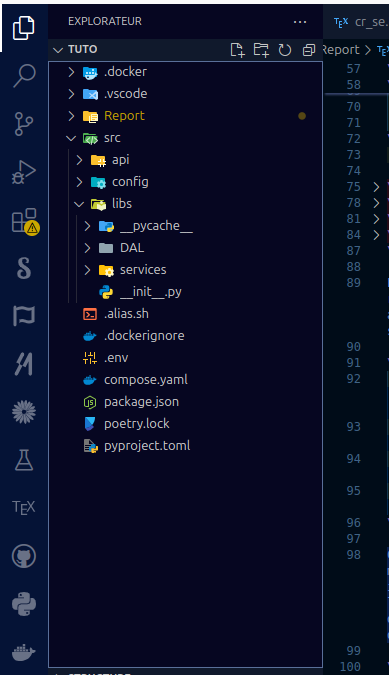
\includegraphics[width=0.45\textwidth]{architecture.png}
  \caption{Architecture du projet avec Docker et bases NoSQL}
  \label{fig:architecture}
\end{figure}


\section{Stratégie de Migration de SQL vers NoSQL}
La base de données SQL originale se composait de plusieurs tables interconnectées qui suivaient un modèle relationnel strict. Cependant, ce modèle, bien que robuste pour certains cas d’utilisation, a montré ses limites dans la gestion des données dynamiques et évolutives. Cela nous a conduit à prendre la décision de passer à une architecture NoSQL, plus adaptée aux besoins actuels.

Le schéma suivant illustre la structure de la base SQL avant migration: 

\begin{figure}[H]
  \centering
  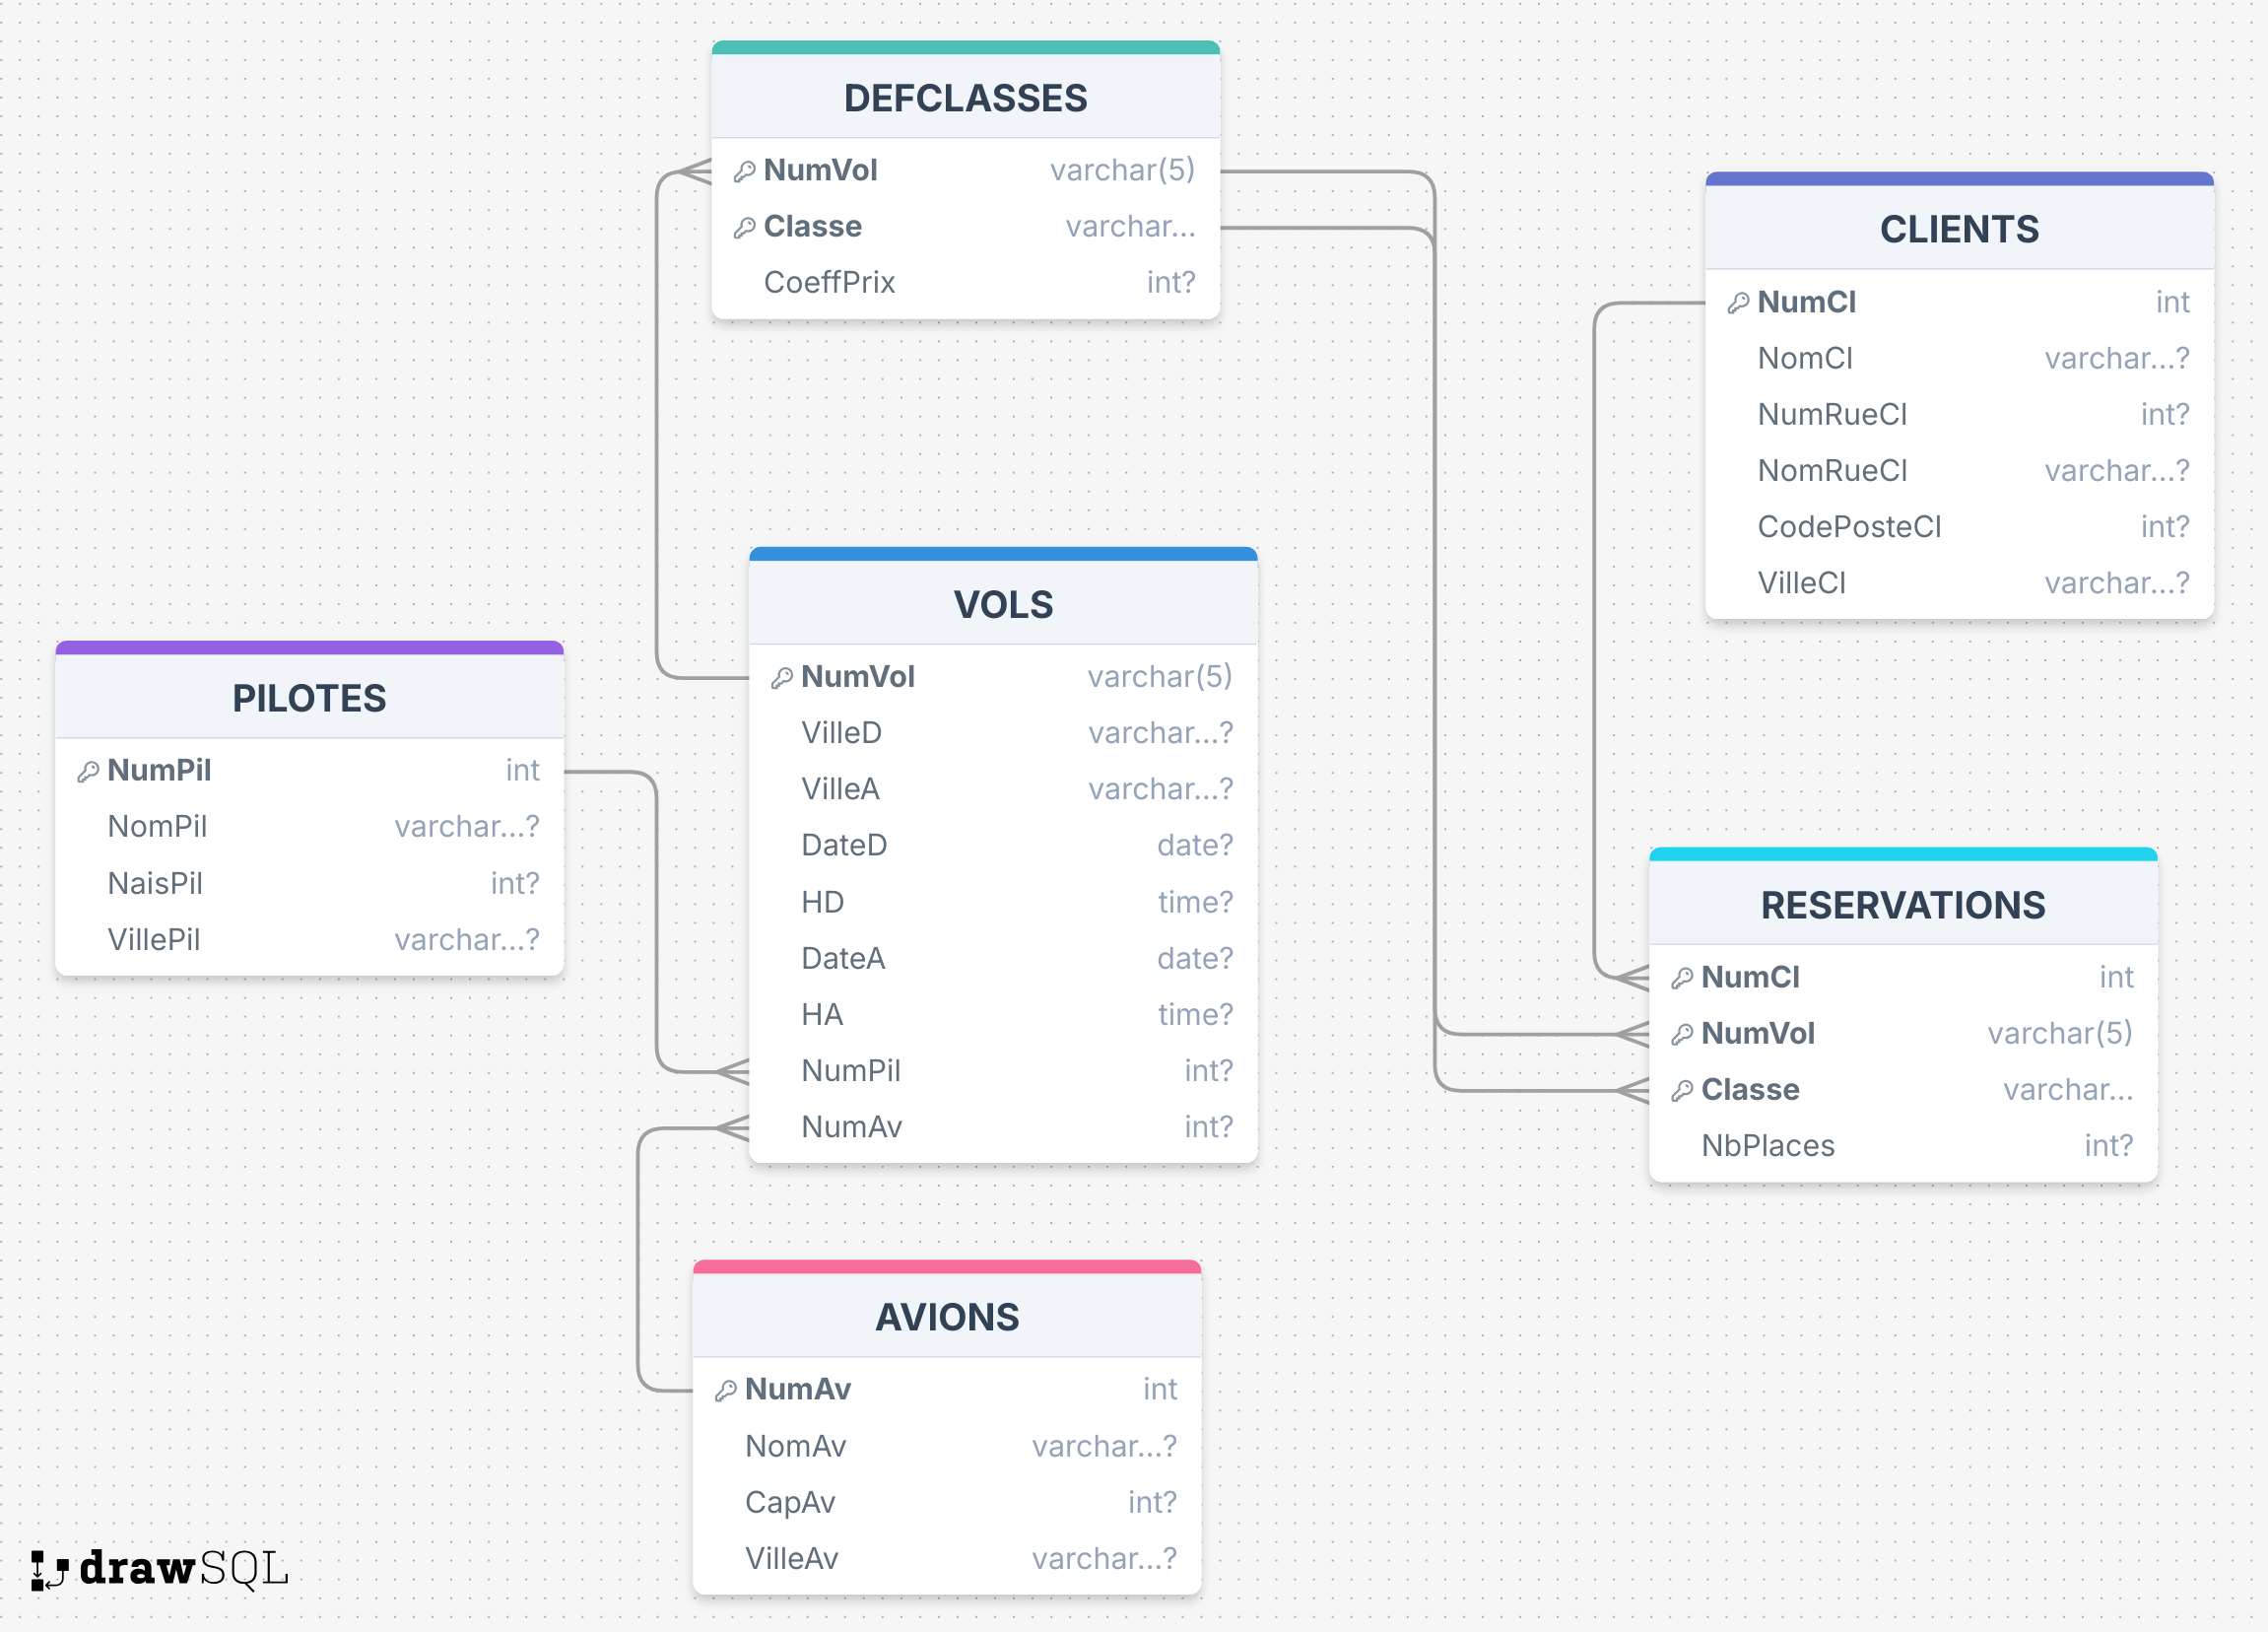
\includegraphics[width=0.8\textwidth]{schema.png}
  \caption{Schéma de la base SQL}
\end{figure}

\subsection{Étape 1:Regroupement des informations de Vols, Avions et Pilotes}

Dans le modèle SQL, pour récupérer toutes les informations d'un vol, il était nécessaire de joindre les tables `VOLS', `AVIONS' et `PILOTES', car chaque table stockait les données d'une entité spécifique. Par exemple, la table `VOLS' contenait les informations sur le vol, mais il fallait ensuite faire une jointure avec `AVIONS' pour connaître les détails de l'avion, et avec `PILOTES' pour obtenir les informations du pilote.

En NoSQL, nous avons choisi de regrouper toutes ces informations dans un seul document au sein de la collection `Vols`. Cette approche permet de conserver toutes les données pertinentes pour un vol dans un seul document JSON.\@

\begin{verbatim}
Vol = {
  _id : 'V001',
  VilleD : 'Paris',
  VilleA : 'New York',
  DateD : '2024-12-01',
  HD : '08:00',
  DateA : '2024-12-01',
  HA : '14:00',
  Avion : { ... },
  Pilote : { ... }
}
\end{verbatim}

Ce choix a été motivé par plusieurs raisons:
\begin{itemize}
  \item \textbf{Élimination des jointures}: En SQL, récupérer ces informations nécessitait de multiples jointures. En NoSQL, en regroupant ces informations dans un seul document, nous réduisons considérablement le coût des requêtes.
  \item \textbf{Accès optimisé aux données}: Toutes les données relatives à un vol, un avion et un pilote étant dans un seul document, cela permet un accès plus rapide et plus direct.
  \item \textbf{Regroupement logique}: Les informations sur les vols, les avions et les pilotes sont souvent interrogées ensemble, il est donc logique de les stocker ensemble.
\end{itemize}

\subsection{Étape 2:Intégration des Classes de Vols}

Dans la base SQL, les différentes classes de service (`Economy', `Business') étaient stockées dans une table séparée appelée `DEFCLASSES',\@ et elles étaient liées à la table `VOLS' par le numéro de vol. Cela nécessitait une jointure supplémentaire pour récupérer les informations des classes disponibles pour chaque vol.

Dans le modèle NoSQL, nous avons décidé d’inclure les classes disponibles directement dans une liste au sein du document `Vol`. Chaque élément de cette liste contient la classe (`Economy', `Business') ainsi que son coefficient de prix.

\begin{verbatim}
  /* Classes disponibles pour le vol */
  Classes : [
    {
      Classe : 'Economy',
      CoeffPrix : 1.0
    },
    {
      Classe : 'Business',
      CoeffPrix : 1.5
    }
  ]
\end{verbatim}

Ce choix s'explique par les avantages suivants:
\begin{itemize}
  \item \textbf{Simplification des requêtes}: En incluant les informations des classes directement dans le document `Vol', nous évitons d’avoir à effectuer une jointure supplémentaire pour les récupérer.
  \item \textbf{Centralisation des données du vol}: Toutes les informations pertinentes concernant un vol (y compris les classes de service) sont désormais disponibles en une seule requête.
  \item \textbf{Flexibilité du modèle NoSQL}: Le format JSON nous permet de structurer ces informations sous forme de liste, ce qui correspond bien à la nature dynamique des classes de vol, et permet d’ajouter facilement de nouvelles classes si nécessaire.
\end{itemize}

\subsection{Étape 3:Gestion des Clients}

Dans le modèle SQL, la table `CLIENTS' stockait des informations sur les clients, notamment leur nom, adresse, et autres coordonnées. Les champs d'adresse (numéro de rue, nom de rue, code postal, ville) étaient représentés par plusieurs colonnes.

Dans la structure NoSQL, nous avons décidé d'imbriquer les informations d'adresse dans un sous-document appelé `Adresse' pour chaque document `Client'.

\begin{verbatim}
Client = {
  _id : 789,
  NomCl : 'Alice Dupont',
  Adresse : { ... },
  Email : 'alice.dupont@example.com',
  Telephone : '0123456789'
}
\end{verbatim}

Ce choix a été fait pour les raisons suivantes:
\begin{itemize}
  \item \textbf{Regroupement logique des informations}: En imbriquant les informations d'adresse dans un sous-document, nous améliorons la cohérence et la gestion des données.
  \item \textbf{Flexibilité}: Si des champs supplémentaires liés à l’adresse sont nécessaires à l’avenir (comme le pays ou la région), ils peuvent être ajoutés sans avoir à modifier toute la structure.
\end{itemize}

\subsection{Étape 4:Représentation des Réservations}

Dans la base SQL, la table `RESERVATIONS' établissait des relations entre les clients et les vols via des clés étrangères, reliant également les classes de service. Dans le modèle NoSQL, nous avons conservé ce concept de relation en utilisant des identifiants (`VolId' et `ClientId') pour relier les documents `Reservation' aux documents `Vol' et `Client'.

\begin{verbatim}
Reservation = {
  _id : 'R001',
  VolId : 'V001',
  ClientId : 789,
  NbPlaces : 2,
  Classe : 'Economy'
}
\end{verbatim}

Nous avons fait ce choix pour les raisons suivantes:
\begin{itemize}
  \item \textbf{Conservation des relations critiques}: Même dans un modèle NoSQL, certaines relations doivent être maintenues. Ici, nous utilisons des identifiants pour lier les réservations aux vols et aux clients sans dupliquer inutilement les données.
  \item \textbf{Économie de stockage}: En stockant uniquement les références aux documents `Vol' et `Client', nous évitons de dupliquer les informations des vols et des clients dans chaque réservation.
\end{itemize}

\section{Conversion des données TXT en JSON}

Le script~\ref{ann:code_json} montre la création de 3 documents json a partir de nos 6 tables, ces tables peuveut être intégré facilement à Redis en ayant comme index le nom de la collection et indice (id) et pour mongo cela peut être représenté en trois collections chacune avec ses documents.\@ et chaque document a un id unique.

\subsection{Insertion des documents dans Redis}

Pour insérer les documents dans Redis nous utiliserons le script~\ref{ann:redis_insert} qui charge les données JSON, les insère dans Redis et affiche un message de succès.

la figure \ref{fig:redis_insert} représente la sortie de la commande \texttt{redis-cli} qui affiche les données insérées dans Redis.

\begin{figure}[H]
  \centering
  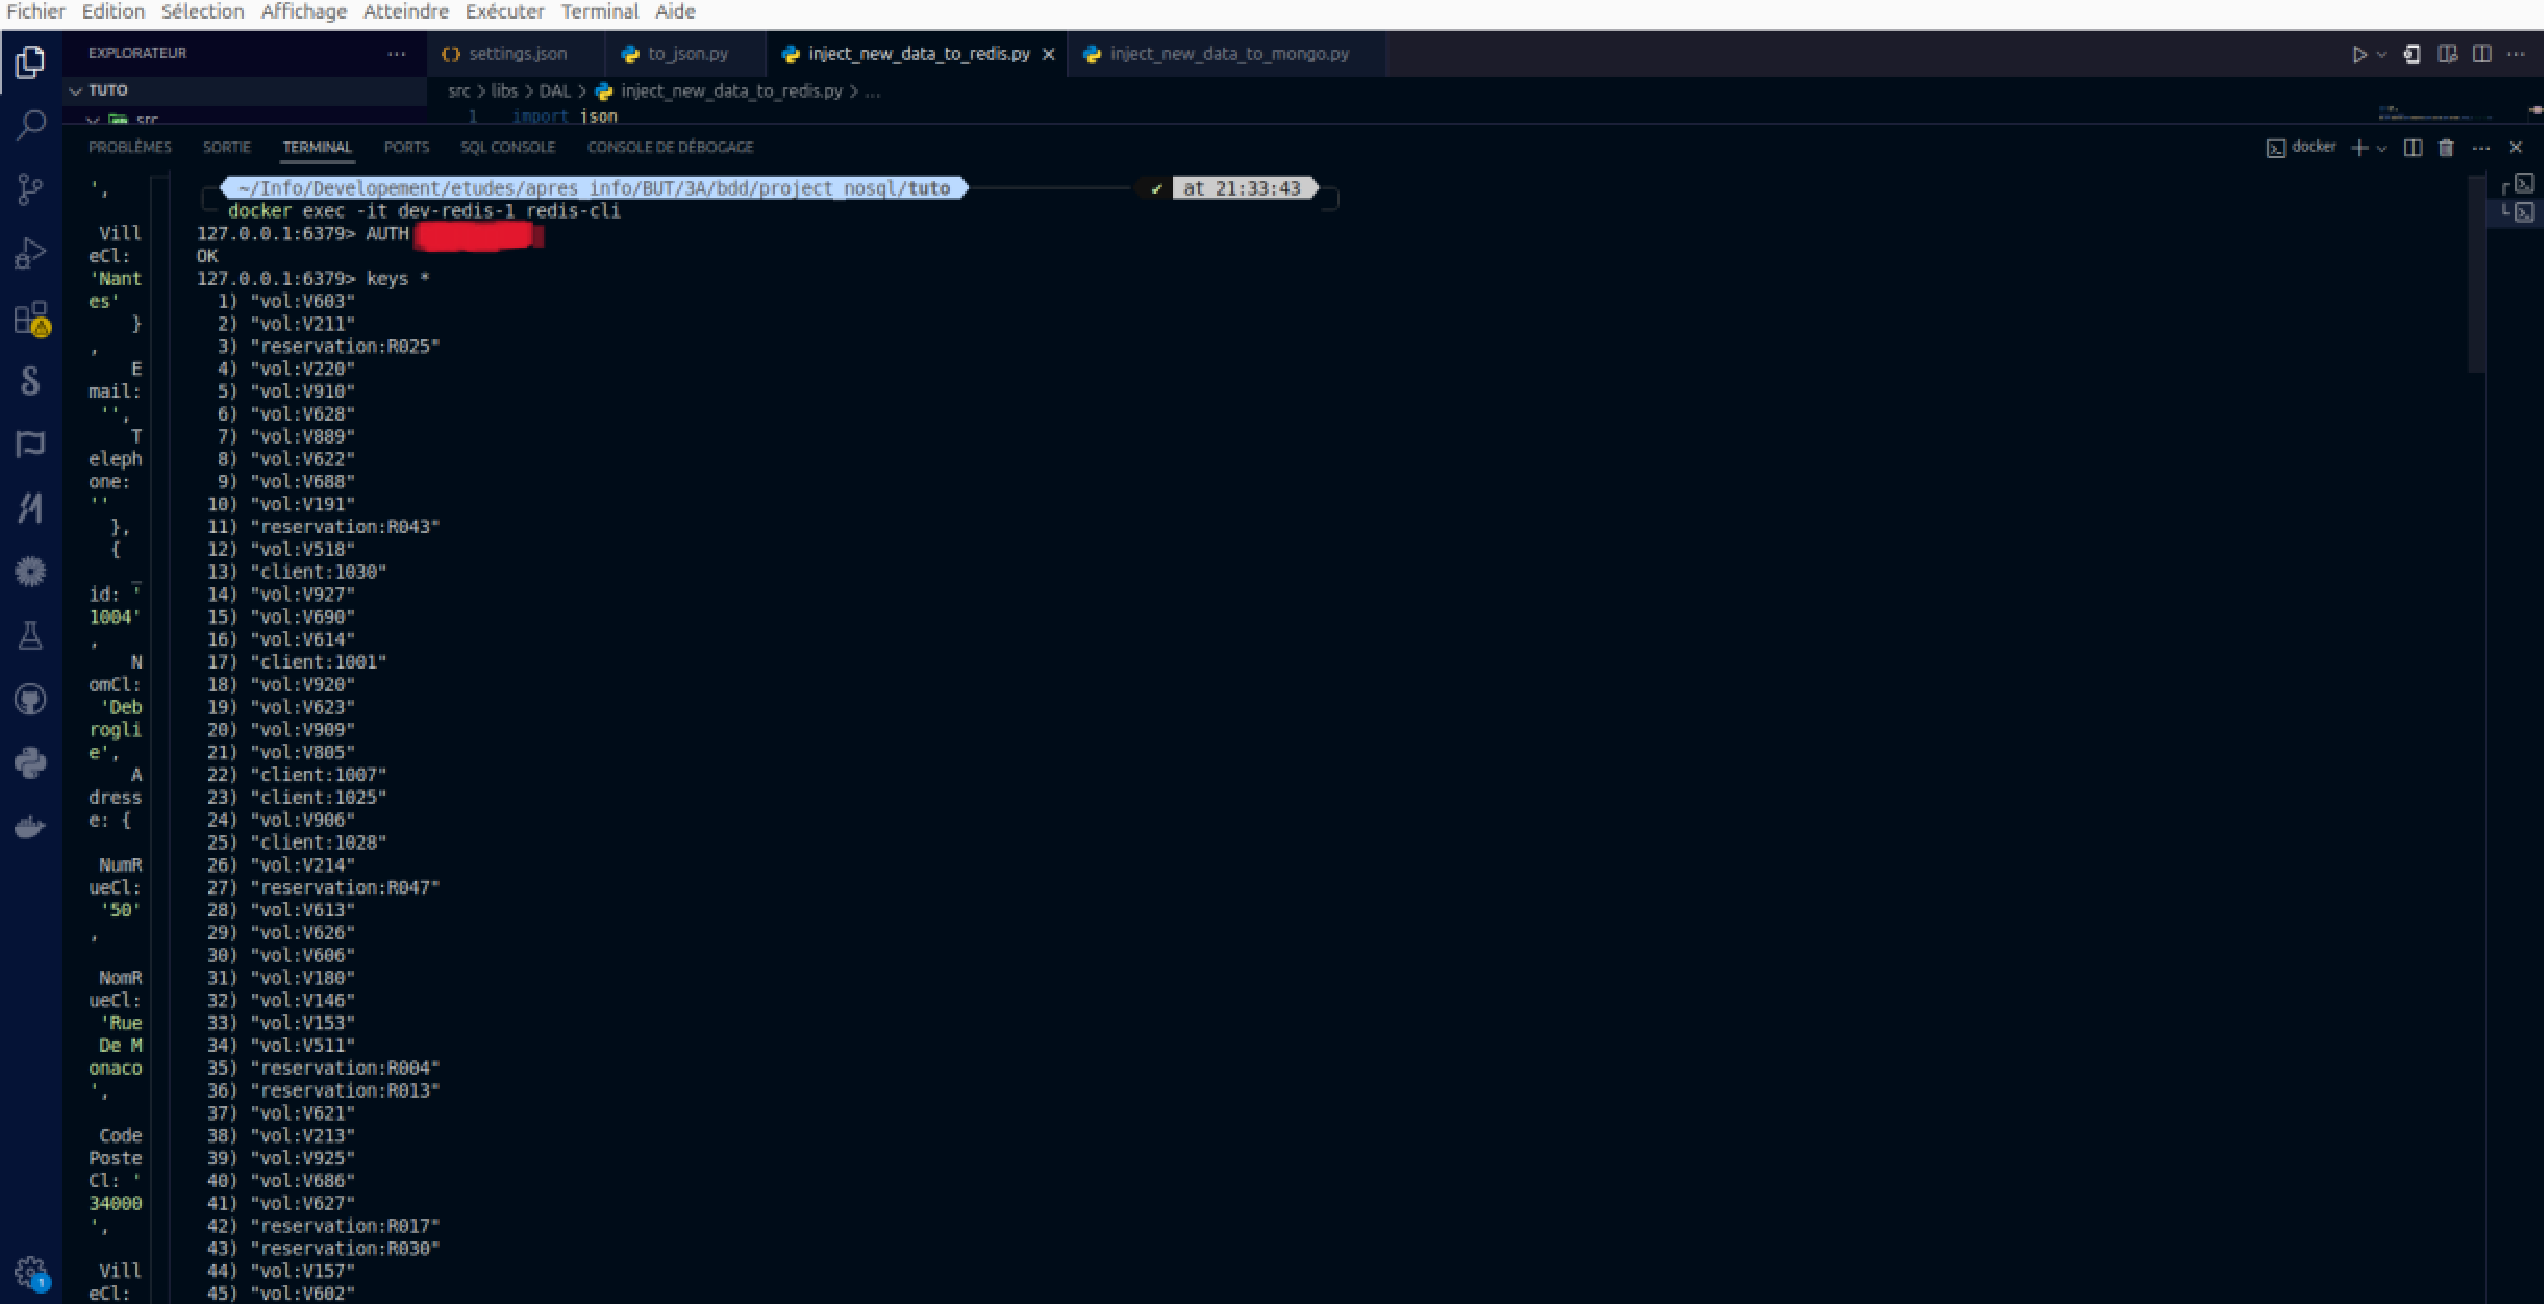
\includegraphics[width=1\textwidth]{redis.pdf}
  \caption{Insertion des documents dans Redis}
  \label{fig:redis_insert}
\end{figure}

\subsection{Insertion des documents dans MongoDB}

Pour insérer les documents dans MongoDB nous utiliserons le script~\ref{ann:mongo_insert} qui charge les données JSON, les insère dans MongoDB et affiche un message de succès.

la figure~\ref{fig:mongo_insert} représente la sortie de la commande \texttt{mongo} qui affiche les données insérées dans MongoDB.\@

\begin{figure}[H]
  \centering
  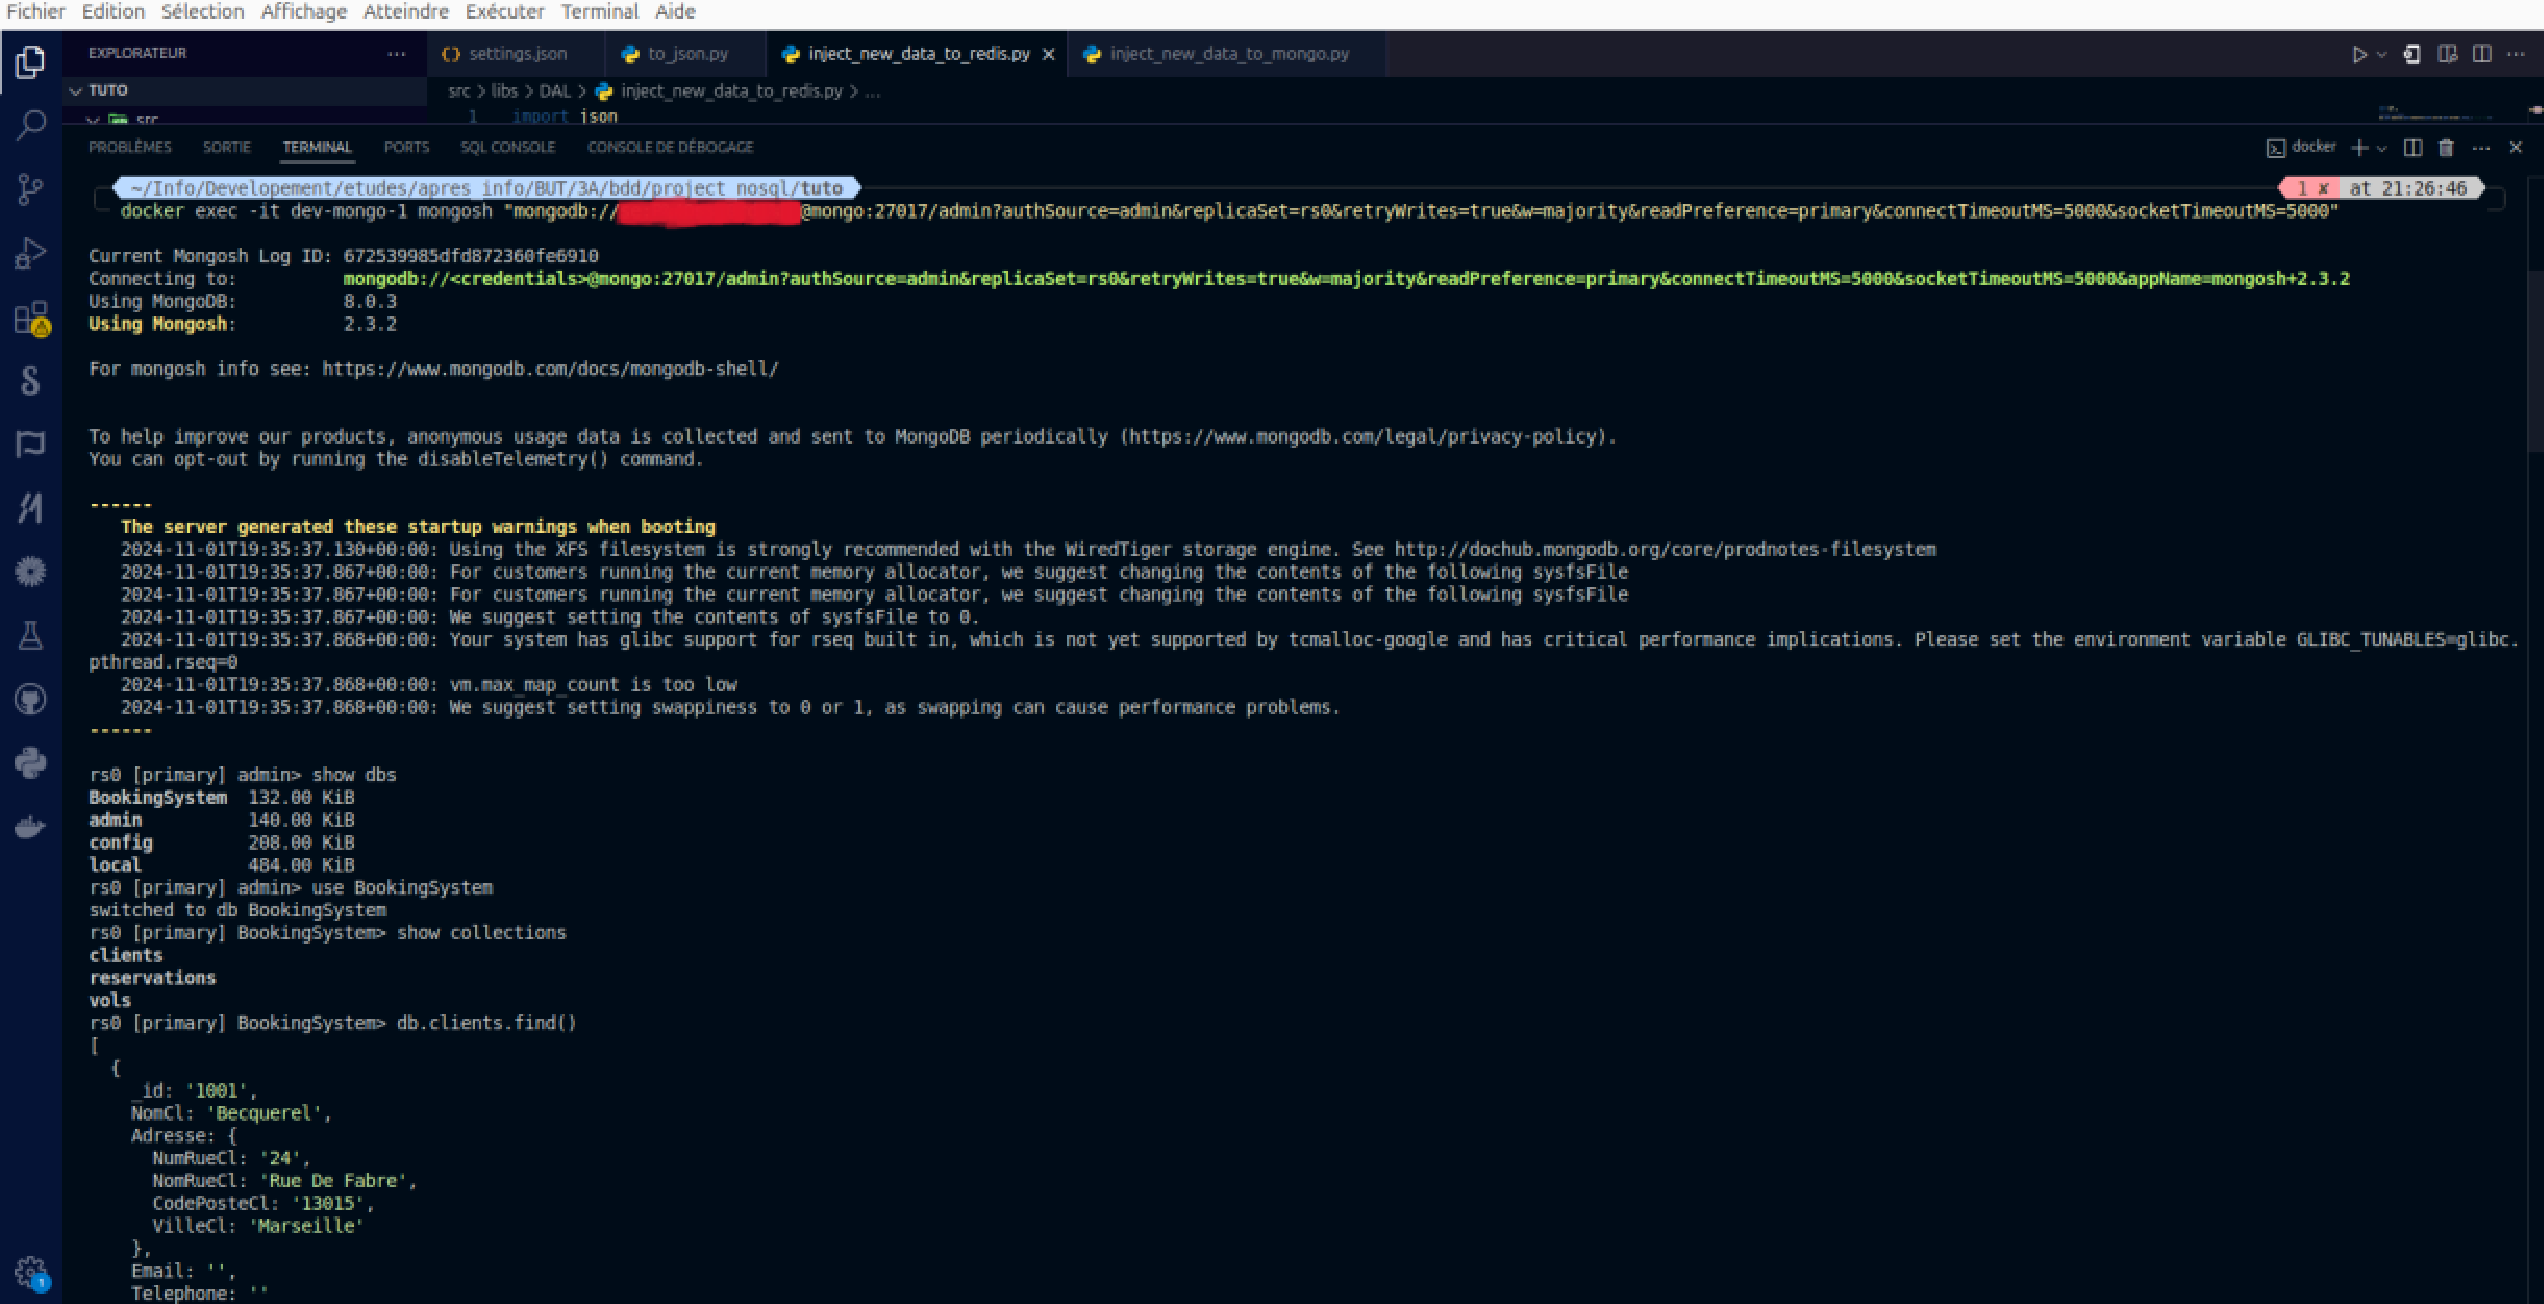
\includegraphics[width=1\textwidth]{mongo.pdf}
  \caption{Insertion des documents dans MongoDB}
  \label{fig:mongo_insert}
\end{figure}
% Résultats
\chapter{Résultats}
Les résultats de la migration sont présentés sous forme de documents JSON pour chaque entité, illustrant les avantages de la dénormalisation et les structures simplifiées obtenues. On peut visualiser les résultats en effectuant des requetes vers la base de données NoSQL et donc au JSON car le format JSON est utilisé dans redis et mongo en tant que document.

Pour illustrer les avantages de la dénormalisation, nous avons utilisé des exemples de requêtes et de jointures pour montrer comment les données peuvent être manipulées et agrégées de manière plus efficace. Ces exemples sont présentés dans la section suivante.

\section{Réplication des résultats}

Avec MongoDB, nous avons mis en place un système de réplication entre trois serveurs pour garantir un accès continu à nos données. Cela permet aussi de réduire les temps de chargement des données, car les données sont chargées de manière asynchrone sur les serveurs. On peux voir dans~\ref{lst:docker_mongo} la configuration des serveurs MongoDB et dans~\ref{lst:replica_set} le script de réplication qui montre comment on ajoute un serveur supplémentaire à la réplication en tant que membres.

\section{Exemple de requêtes et de jointures}

En ayant convertit nos tables SQL en JSON, nous pouvons normaliser les requêtes et les jointures pour manipuler les données de manière plus efficace que les données viennent d'un fichier JSON, récupéré par redis ou par mongo.

On peux voir dans~\ref{lst:results_queries} les résultats des requêtes avec les données d'origine et le résultat des requêtes est le meme pour Redis, MongoDB et MONGO\_JSON.\@

\section{Utilisation des ressources matérielles}

Voici les ressources matérielles utilisées pour le développement de ce projet:

\begin{figure}[H]
  \centering
  \begin{subfigure}[t]{0.88\textwidth}
    \centering
    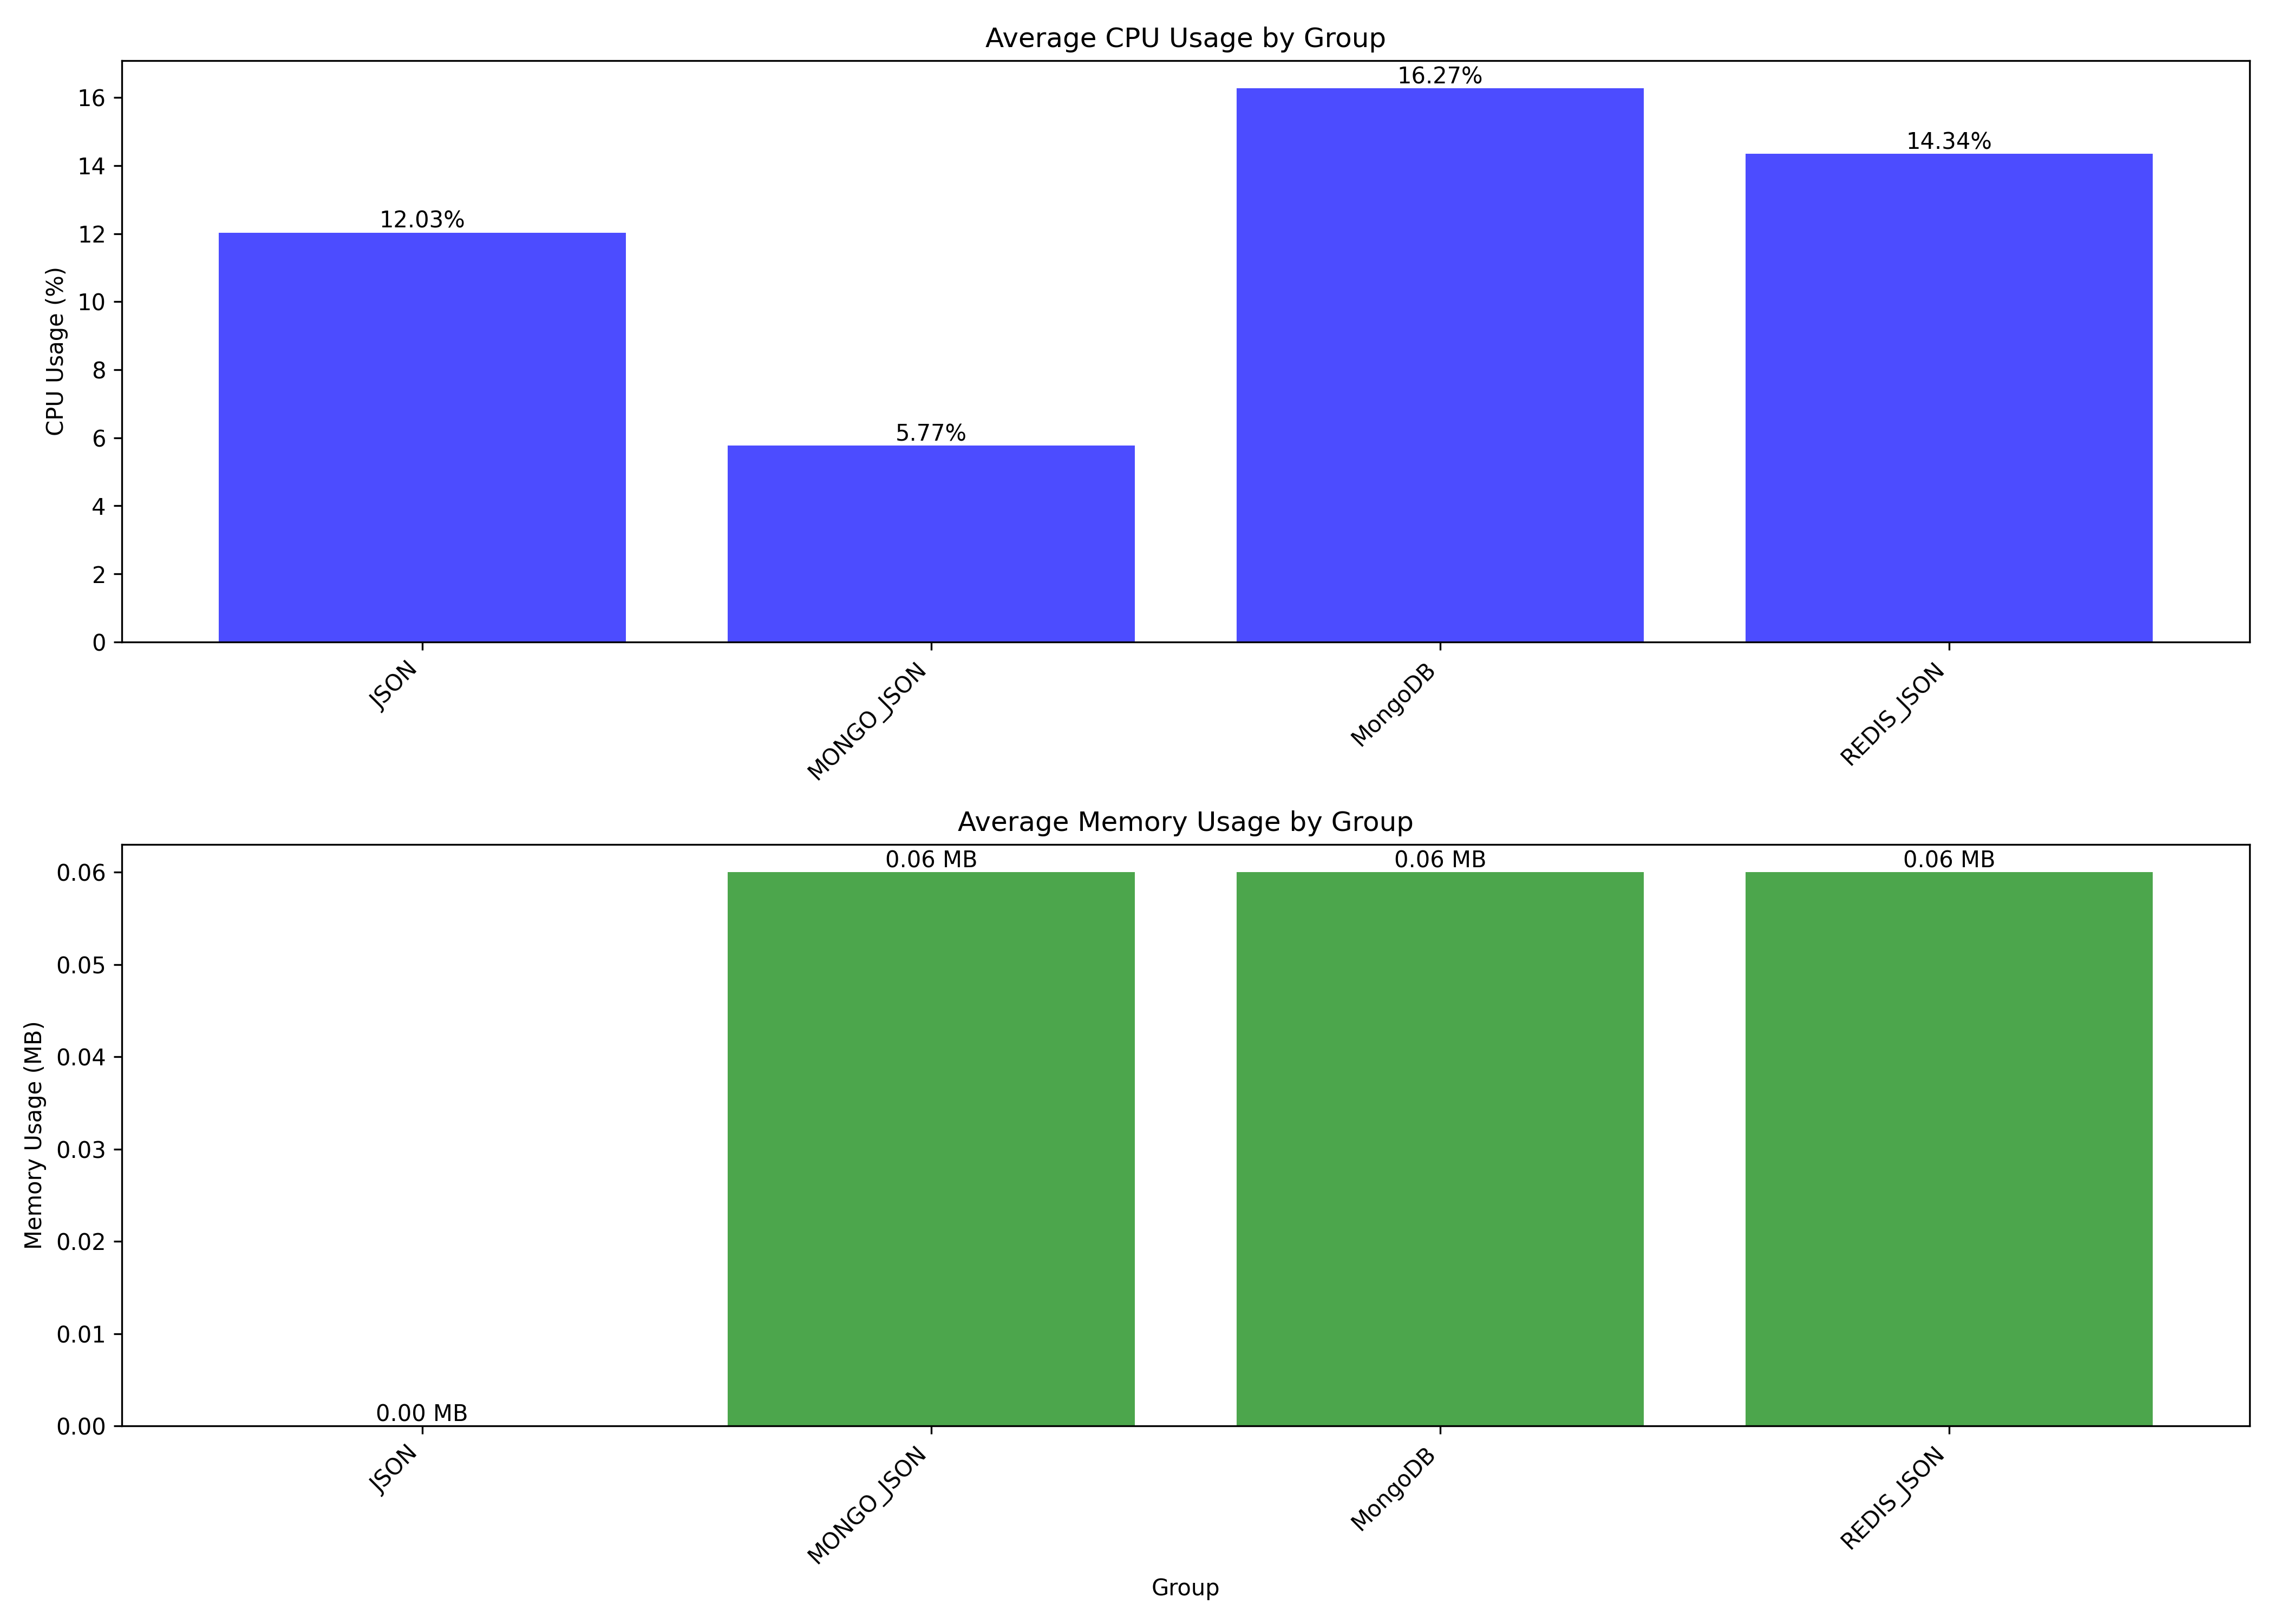
\includegraphics[width=\linewidth]{small/resources_comparison_global_metrics.png}
    \caption{Comparaison des ressources matérielles avec les données d'origine}
    \label{fig:res_origin}
  \end{subfigure}
  \hfill
  \begin{subfigure}[t]{0.88\textwidth}
    \centering
    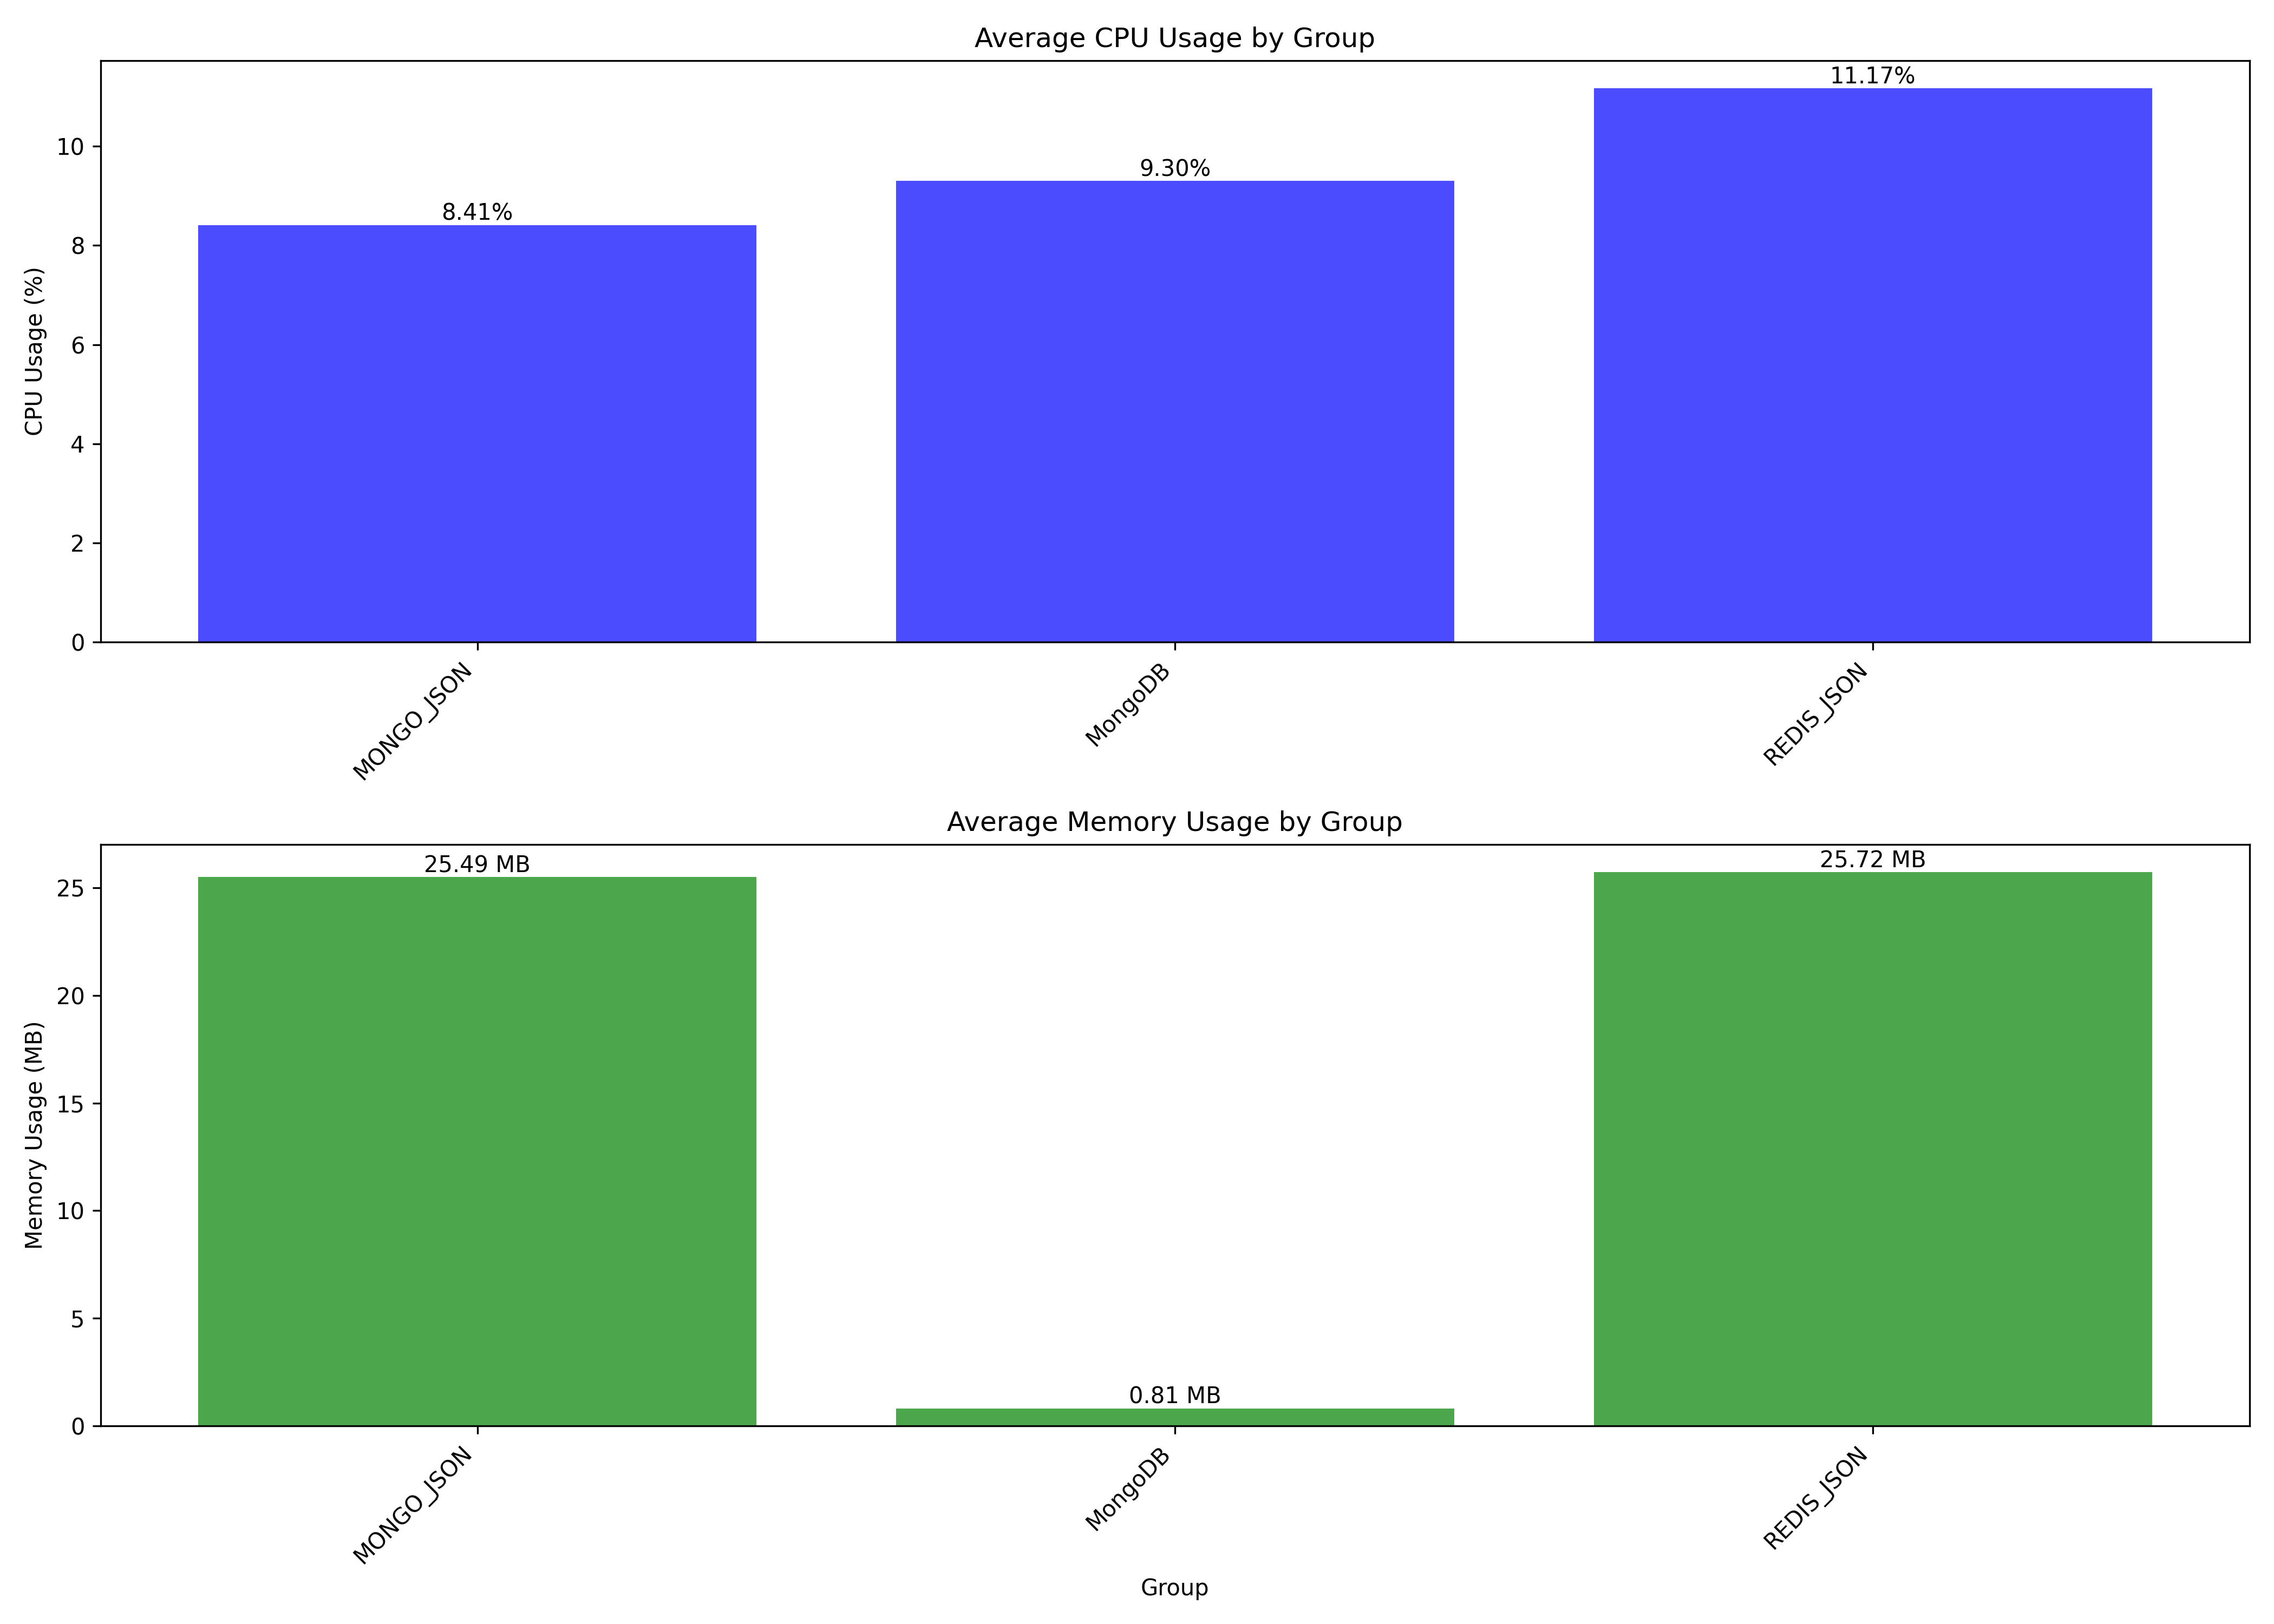
\includegraphics[width=\linewidth]{resources_comparison_global_metrics.png}
    \caption{Comparaison des ressources matérielles avec un grand volume de données}
    \label{fig:res_total}
  \end{subfigure}
  \caption{Comparaison des ressources matérielles utilisées avec les données d'origine et avec un grand volume de données}
  \label{fig:comparaison_resources}
\end{figure}

\section{Comparaison des Performances}

La figure~\ref{fig:origin} montre les performances des requêtes avec les données d'origine, tandis que la figure~\ref{fig:total} montre les performances avec un grand volume de données.

On peut voir que pour un nombre de données faibles, le temps de requêtes avec Redis en important en JSON est plus faible que avec MongoDB en JSON et avec des recherches MongoDB (Pipelines). Cependant, avec un volume de données plus important, les performances sont plus élevées avec MongoDB (Pipelines) et en stocker les données Mongo en JSON.\@

\begin{figure}[H]
  \centering
  \begin{subfigure}[t]{0.45\textwidth}
    \centering
    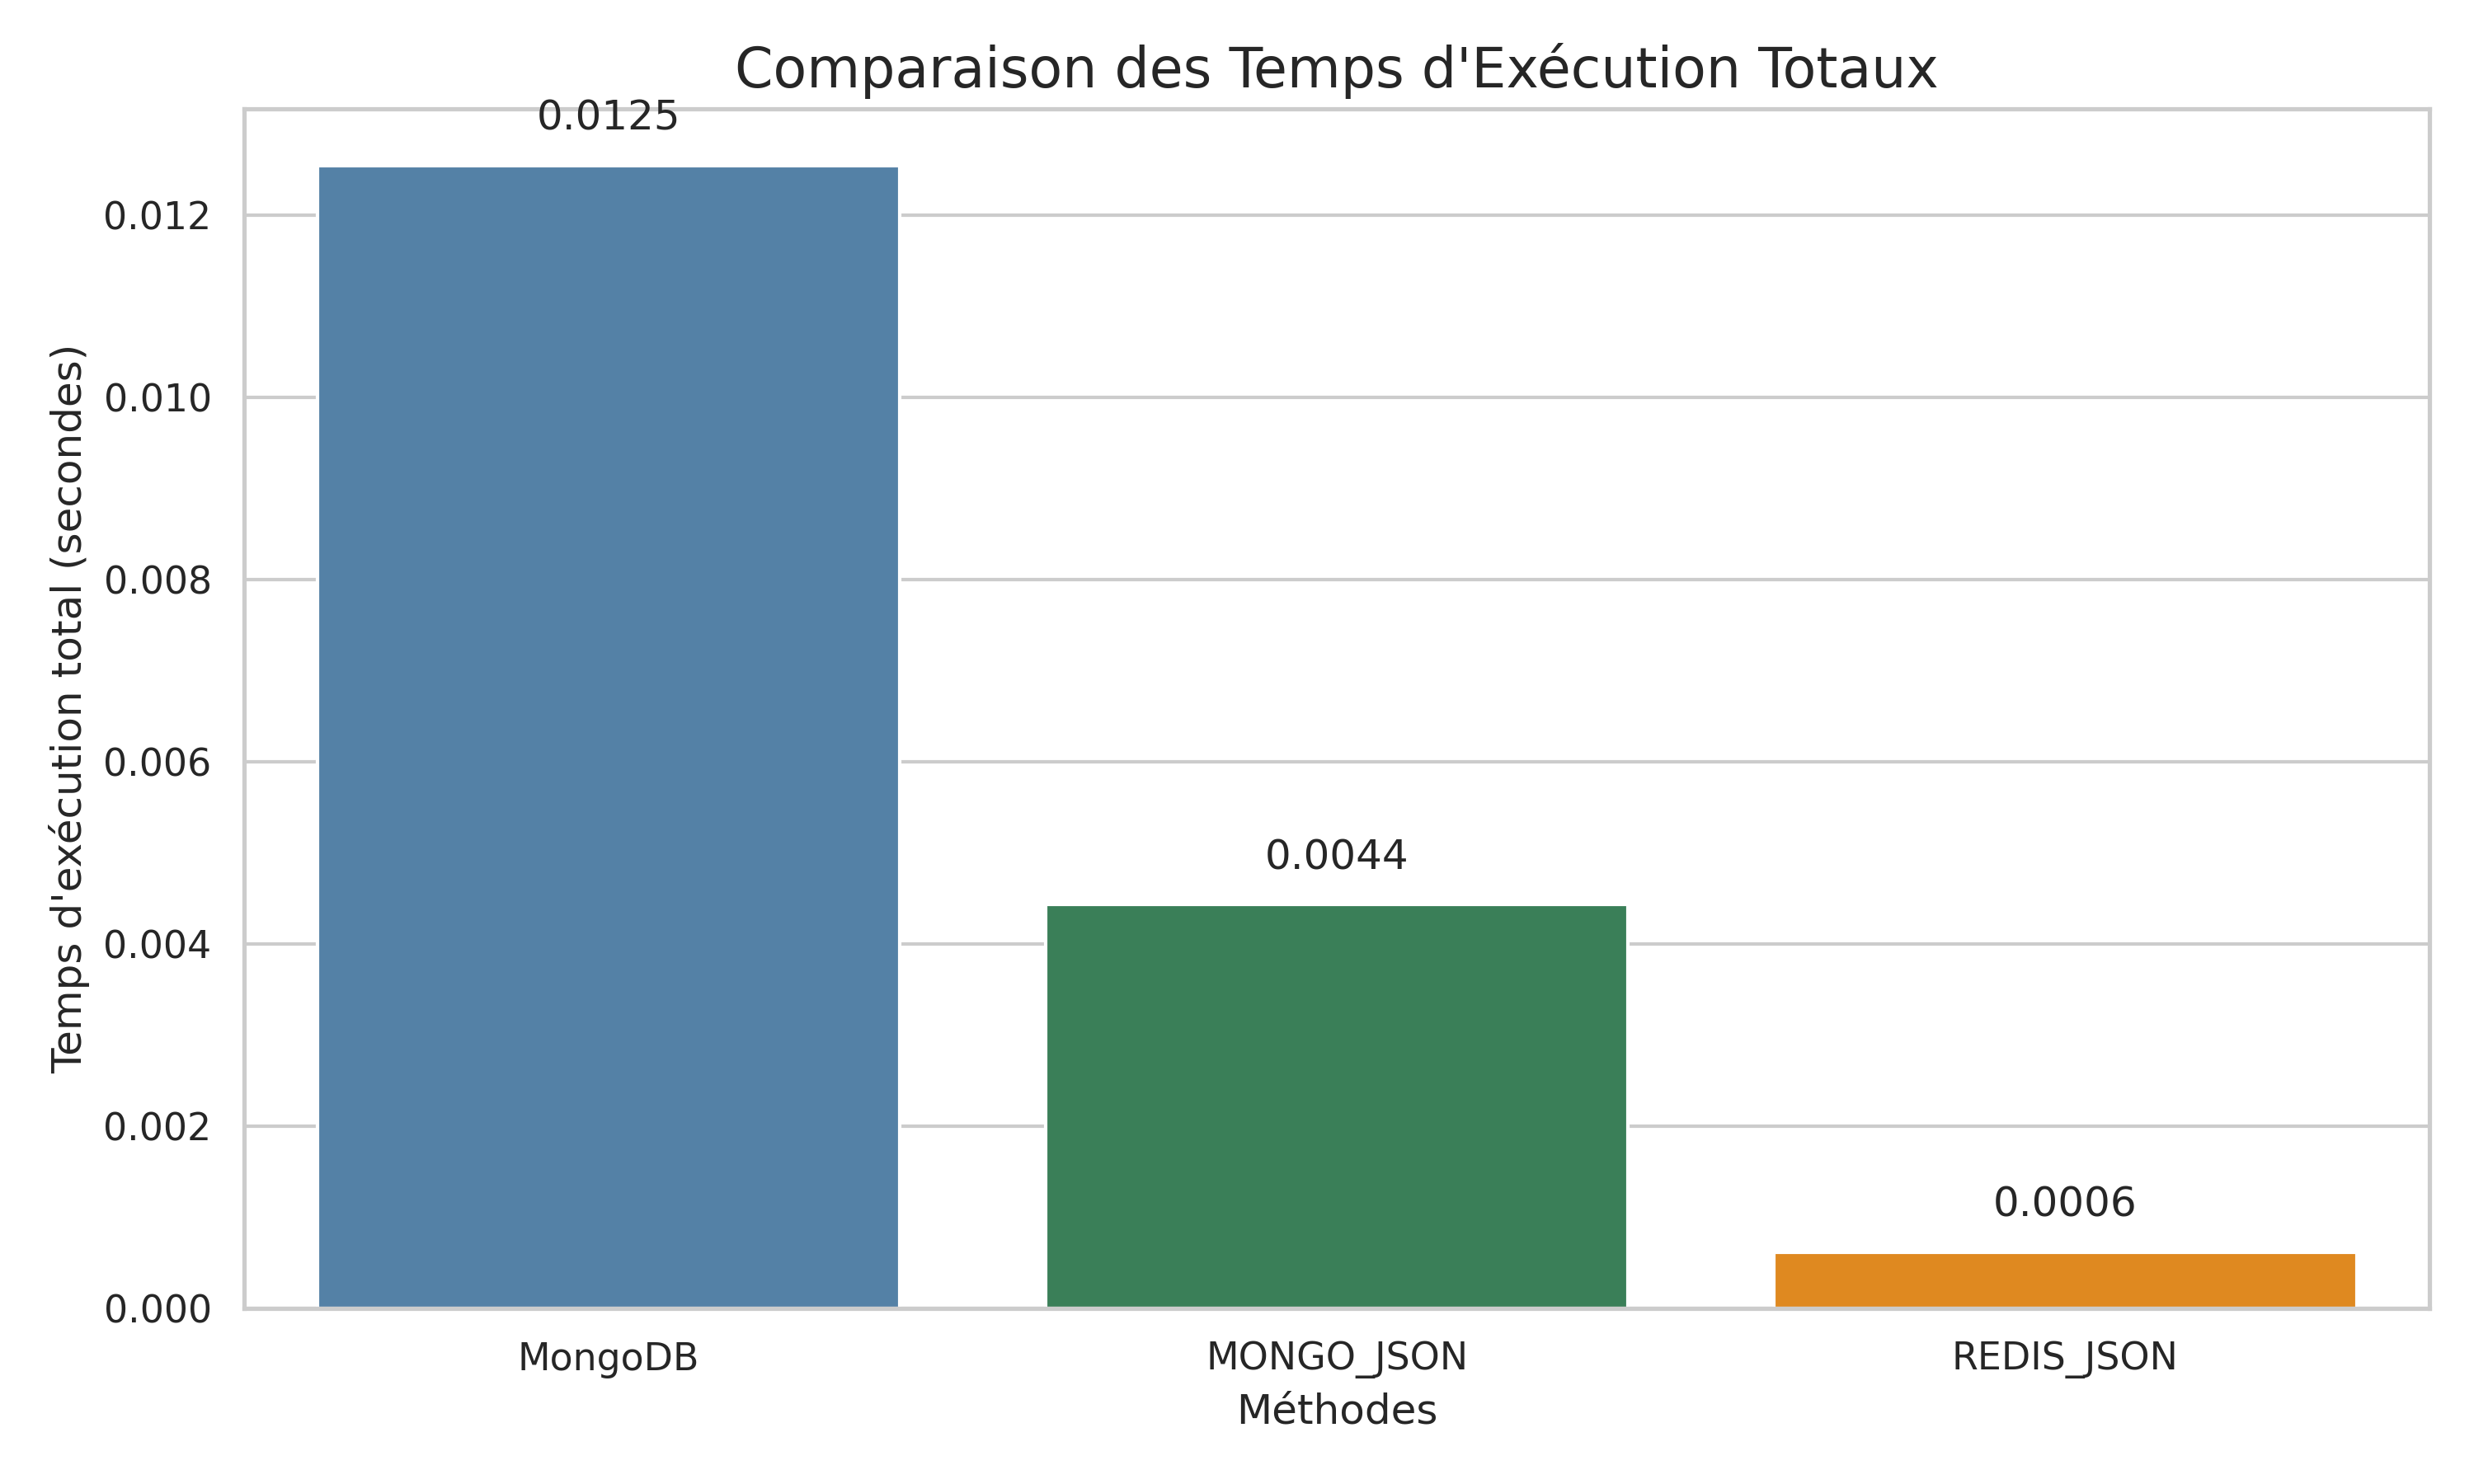
\includegraphics[width=\linewidth]{small/execution_times_comparison_total.png}
    \caption{Comparaison des performances avec les données d'origine}
    \label{fig:origin}
  \end{subfigure}
  \hfill
  \begin{subfigure}[t]{0.45\textwidth}
    \centering
    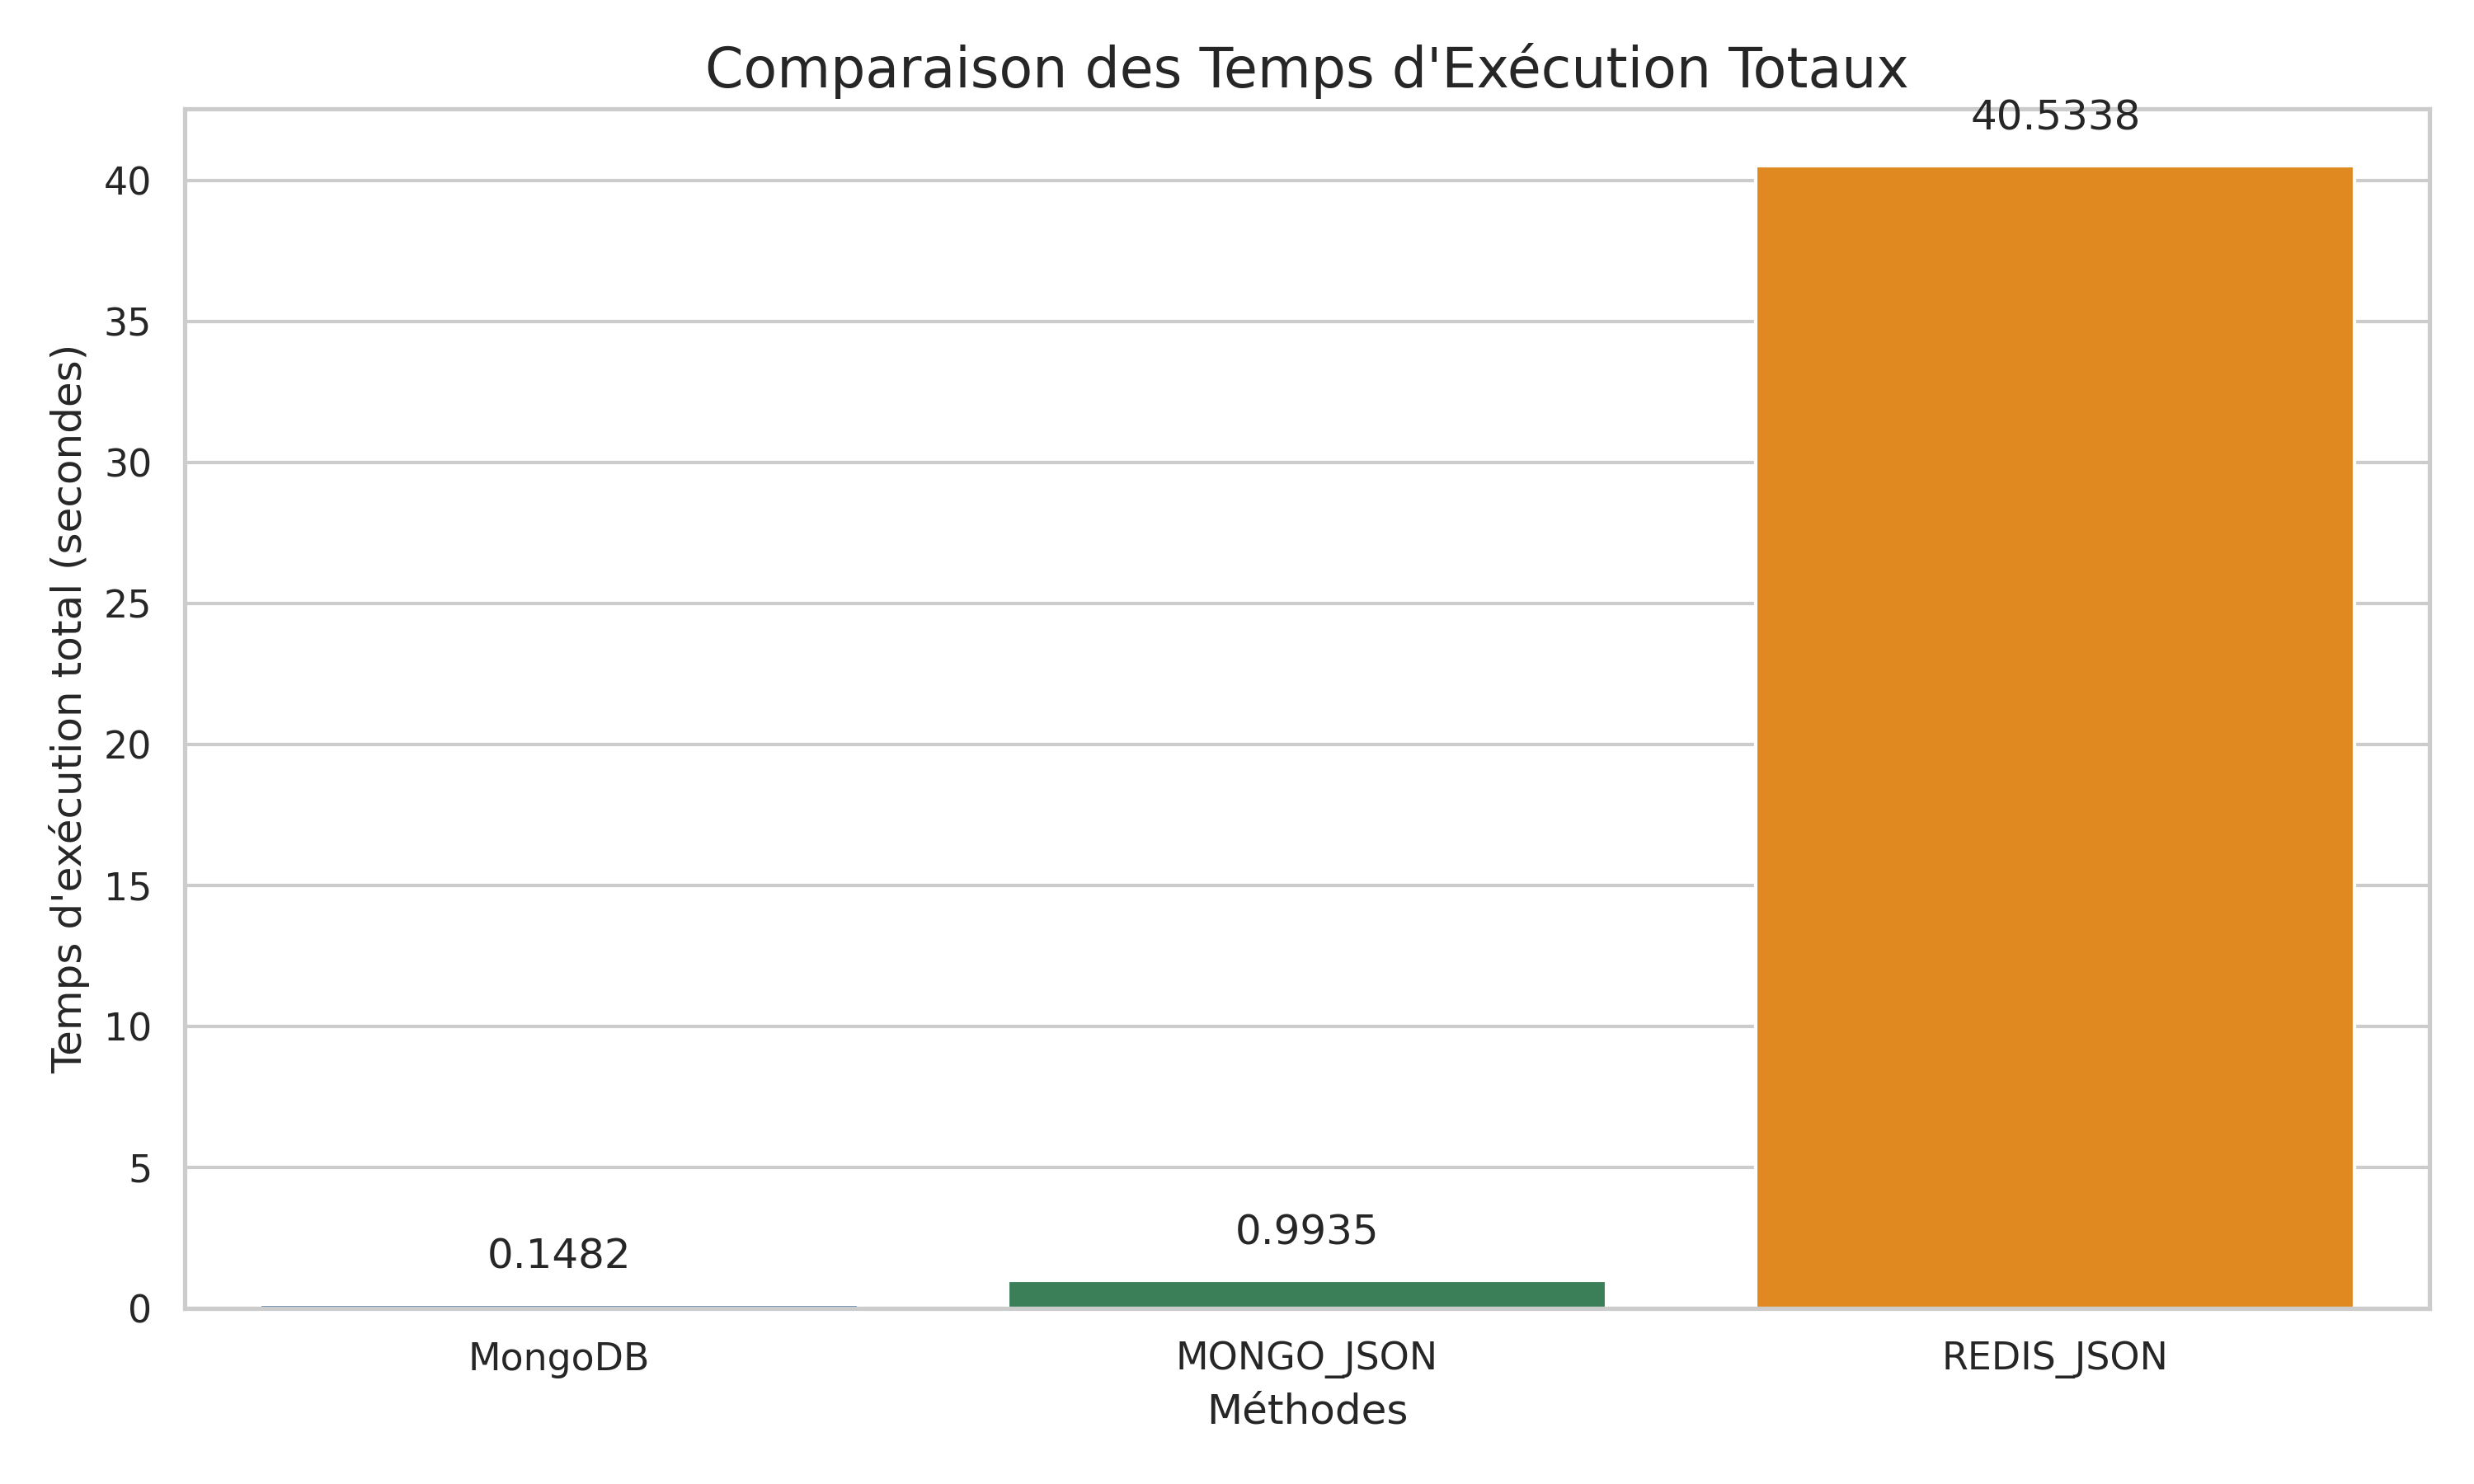
\includegraphics[width=\linewidth]{execution_times_comparison_total.png}
    \caption{Comparaison des performances avec un grand volume de données}
    \label{fig:total}
  \end{subfigure}
  \caption{Comparaison des performances avec les données d'origine et avec un grand volume de données}
  \label{fig:comparaison_performances}
\end{figure}

% Discussion
\chapter{Discussion}
Cette section analyse comment les résultats de la migration répondent aux objectifs fixés et aux besoins d’optimisation des performances. Nous avons mesuré les performances de chaque base de données à travers plusieurs requêtes (profiling détaillé en annexe~\ref{ann:profiling}).

\section{Comparaison des Performances}
Les résultats montrent que Redis offre des temps de réponse plus rapides pour les opérations de lecture, tandis que MongoDB est plus adapté pour les requêtes complexes grâce à son système de stockage JSON natif.

\begin{table}[htbp]
  \centering
  \caption{Comparaison des performances entre MongoDB, MONGO\_JSON et REDIS\_JSON}
  \label{tab:performance1}
  \begin{adjustbox}{width=\textwidth}
  \begin{tabular}{lccccccc}
  \toprule
  \textbf{Fonction} & \textbf{Temps MongoDB} & \textbf{Temps MONGO\_JSON} & \textbf{Temps REDIS\_JSON} & \textbf{Diff MONGO\_JSON} & \textbf{Diff REDIS\_JSON} & \textbf{\% Diff MONGO\_JSON} & \textbf{\% Diff REDIS\_JSON} \\
  \midrule
  get\_flights\_by\_pilot       & 0.001110 & 0.000065 & 0.000002 & -0.001046 & -0.001109 & -94.17\%  & -99.84\%  \\
  get\_reservations\_by\_client & 0.001186 & 0.000015 & 0.000003 & -0.001171 & -0.001183 & -98.75\%  & -99.74\%  \\
  get\_clients\_by\_flight      & 0.000767 & 0.000010 & 0.000003 & -0.000757 & -0.000764 & -98.68\%  & -99.66\%  \\
  get\_vols\_by\_departure\_city & 0.001531 & 0.000080 & 0.000003 & -0.001451 & -0.001529 & -94.76\%  & -99.81\%  \\
  load\_data\_from\_mongo       & N/A      & 0.003973 & N/A       & N/A       & N/A       & N/A       & N/A       \\
  get\_clients\_by\_pilot       & 0.005947 & 0.000136 & 0.000021 & -0.005811 & -0.005927 & -97.71\%  & -99.65\%  \\
  load\_data\_from\_redis       & N/A      & N/A      & 0.000578 & N/A       & N/A       & N/A       & N/A       \\
  get\_arrival\_cities          & 0.000921 & 0.000015 & 0.000002 & -0.000906 & -0.000919 & -98.38\%  & -99.81\%  \\
  get\_pilotes                  & 0.000541 & 0.000103 & 0.000005 & -0.000437 & -0.000535 & -80.88\%  & -99.01\%  \\
  get\_arrival\_city\_by\_id     & 0.000541 & 0.000034 & 0.000002 & -0.000508 & -0.000540 & -93.73\%  & -99.64\%  \\
  \midrule
  \textbf{Total}                & \textbf{0.012545} & \textbf{0.004432} & \textbf{0.000618} & \textbf{-0.008113} & \textbf{-0.011927} & \textbf{-64.67\%} & \textbf{-95.08\%} \\
  \bottomrule
  \end{tabular}
  \end{adjustbox}
\end{table}

\begin{table}[htbp]
  \centering
  \caption{Comparaison des performances avec un grand volume de données}
  \label{tab:performance2}
  \begin{adjustbox}{width=\textwidth}
  \begin{tabular}{lccccccc}
  \toprule
  \textbf{Fonction} & \textbf{Temps MongoDB} & \textbf{Temps MONGO\_JSON} & \textbf{Temps REDIS\_JSON} & \textbf{Diff MONGO\_JSON} & \textbf{Diff REDIS\_JSON} & \textbf{\% Diff MONGO\_JSON} & \textbf{\% Diff REDIS\_JSON} \\
  \midrule
  get\_reservations\_by\_client & 0.000784 & 0.019903 & 0.019361 & 0.019119 & 0.018577 & 2439.85\% & 2370.68\% \\
  get\_clients\_by\_flight      & 0.000775 & 0.018795 & 0.021336 & 0.018020 & 0.020561 & 2324.48\% & 2652.33\% \\
  get\_vols\_by\_departure\_city & 0.000957 & 0.022559 & 0.021597 & 0.021602 & 0.020640 & 2257.32\% & 2156.82\% \\
  get\_flights\_by\_pilot       & 0.002058 & 0.015452 & 0.015755 & 0.013394 & 0.013696 & 650.73\%  & 665.44\%  \\
  load\_data\_from\_redis       & N/A      & N/A      & 40.389436 & N/A       & N/A       & N/A       & N/A       \\
  get\_clients\_by\_pilot       & 0.043849 & 0.045735 & 0.052641 & 0.001886 & 0.008792 & 4.30\%    & 20.05\%   \\
  get\_arrival\_cities          & 0.099761 & 0.012911 & 0.013698 & -0.086850 & -0.086062 & -87.06\%  & -86.27\%  \\
  load\_data\_from\_mongo       & N/A      & 0.858132 & N/A       & N/A       & N/A       & N/A       & N/A       \\
  \midrule
  \textbf{Total}                & \textbf{0.148184} & \textbf{0.993487} & \textbf{40.533824} & \textbf{0.845303} & \textbf{40.385640} & \textbf{570.44\%} & \textbf{27253.76\%} \\
  \bottomrule
  \end{tabular}
  \end{adjustbox}
\end{table}

Les performances des bases de données \textbf{MongoDB}, \textbf{MONGO\_JSON} et \textbf{REDIS\_JSON} ont été évaluées en exécutant plusieurs fonctions clés du système. Les résultats sont présentés dans les Tableaux~\ref{tab:performance1} et \ref{tab:performance2}, et illustrés dans la Figure~\ref{fig:comparaison_performances}.

\subsection{Performances avec le Jeu de Données d'Origine}

Le Tableau~\ref{tab:performance1} présente les temps d'exécution des différentes fonctions avec le jeu de données initial, qui contient un volume de données relativement faible. On constate que \textbf{REDIS\_JSON} offre les temps de réponse les plus rapides pour la majorité des fonctions. Par exemple, la fonction \texttt{get\_flights\_by\_pilot} est exécutée en 0.000002 secondes avec \textbf{REDIS\_JSON}, contre 0.001110 secondes avec \textbf{MongoDB}, ce qui représente une amélioration de 99.84\%.

De même, \textbf{MONGO\_JSON} montre des améliorations significatives par rapport à \textbf{MongoDB} standard, avec des gains de performance allant jusqu'à 98\%. Ces améliorations sont dues à l'utilisation d'un format JSON dénormalisé, qui réduit le besoin de jointures et permet un accès plus rapide aux données.

\subsection{Performances avec un Grand Volume de Données}

Le Tableau~\ref{tab:performance2} illustre les performances des mêmes fonctions, mais cette fois avec un grand volume de données. Dans ce scénario, les performances de \textbf{REDIS\_JSON} se dégradent considérablement pour certaines fonctions. Par exemple, la fonction \texttt{load\_data\_from\_redis} prend 40.389436 secondes, ce qui est nettement supérieur aux temps observés avec \textbf{MongoDB}.

En revanche, \textbf{MongoDB} démontre une meilleure scalabilité. Les temps d'exécution restent relativement stables malgré l'augmentation du volume de données. La fonction \texttt{get\_clients\_by\_pilot} est exécutée en 0.043849 secondes avec \textbf{MongoDB}, contre 0.052641 secondes avec \textbf{REDIS\_JSON}, indiquant une meilleure performance pour les requêtes complexes sur de grandes bases de données.

\subsection{Interprétation des Résultats}

Ces résultats mettent en évidence plusieurs points clés :

\begin{itemize}
  \item \textbf{REDIS\_JSON} est extrêmement performant pour les opérations de lecture simples et les petits volumes de données grâce à son stockage en mémoire. Cependant, il montre des limitations en termes de scalabilité lorsque le volume de données augmente.
  \item \textbf{MongoDB}, bien que légèrement moins performant sur de petites requêtes, offre une meilleure gestion des grands volumes de données et des requêtes complexes, grâce à sa structure de stockage optimisée et sa capacité à gérer des index efficaces.
  \item \textbf{MONGO\_JSON} combine les avantages de MongoDB avec une structure de données dénormalisée, offrant de bonnes performances sur des volumes de données moyens, mais peut être limité par rapport à MongoDB standard pour des données massives.
\end{itemize}

La Figure~\ref{fig:comparaison_performances} illustre visuellement ces tendances, montrant comment les temps d'exécution évoluent en fonction du volume de données pour chaque base de données. On y observe que si \textbf{REDIS\_JSON} est le plus rapide sur des petits volumes, \textbf{MongoDB} devient plus performant à mesure que le volume de données augmente.

\subsection{Conclusion sur le Choix des Bases de Données}

Le choix entre \textbf{MongoDB} et \textbf{REDIS\_JSON} dépend fortement des besoins spécifiques du projet :

\begin{itemize}
  \item Si l'application nécessite des temps de réponse ultra-rapides pour des opérations simples sur de petits volumes de données, \textbf{REDIS\_JSON} est recommandé.
  \item Pour des applications manipulant de grands volumes de données avec des requêtes complexes, \textbf{MongoDB} offre une meilleure performance globale et une scalabilité accrue.
\end{itemize}

Il est donc essentiel de prendre en compte le volume de données et la nature des requêtes lors de la sélection de la base de données appropriée pour une application donnée.

\section{Comparaison des Ressources Matérielles}

La figure~\ref{fig:comparaison_resources} illustre les ressources matérielles utilisées pour le développement de ce projet, en comparant les performances des requêtes avec les données d'origine et avec un grand volume de données. On y observe que les ressources utilisées sont basses pour des requêtes avec mongo pour un volume de données faible et pour un volume de données important, les performances sont plus élevées avec des requêtes complexes et avec des données massives.

\section{Limites et Améliorations Possibles}
En implémentant Redis et mongo on peux voir que les deux ont certaines limites en fonction du nombre de données présents dans la base de données.
Une application peut contenir les 2 types de base de données mais ne contenant pas les mêmes données.

Par exemple:
Si on prend en exemple notre cas d'étude pour les vols... on peux mettre tout ça dans notre base mongo car on aura un nombre très important de données dans la base et si on imagine un système d'authentification a votre système de gestion de vols, on pourra stocker les utilisateurs dans mongo et les sessions d'authentification dans redis car on a un faible stockage de données stockées et redis permet de stocker et faire des requêtes pour une petite gestion de mémoire pour ne pas allourdir le système.

Bien que NoSQL ait permis une flexibilité accrue, certains cas d'utilisation nécessitent encore une réflexion pour l'optimisation des écritures massives. On remarque qu'actuellement entre le SQL et le NoSQL on trouve encore certaines limites, faut essayer de voir un nouveau type de base de données pour répondre à ces limites comme le graph database ou le NewSQL avec CockroachDB.

\chapter{Conclusion}

La migration de bases de données relationnelles SQL vers des solutions NoSQL, en utilisant notamment Redis et MongoDB, s'est avérée être une stratégie efficace pour répondre aux besoins croissants de flexibilité et de performance dans la gestion des données. Ce projet a mis en évidence les avantages significatifs qu'offrent ces technologies pour le stockage et la manipulation de données semi-structurées.

Les principaux résultats obtenus sont les suivants :

\begin{itemize}
  \item \textbf{Optimisation des Performances :} Les tests de performance ont démontré que Redis offre des temps de réponse extrêmement rapides pour les opérations de lecture simples sur de petits volumes de données, grâce à son stockage en mémoire. MongoDB, quant à lui, assure une meilleure performance et une scalabilité accrue pour les requêtes complexes et les grands volumes de données, grâce à son système de gestion de documents JSON natif.

  \item \textbf{Flexibilité Accrue :} La transition vers des bases NoSQL a permis de dénormaliser les données et de les structurer de manière plus flexible. Cette approche facilite l'adaptation aux changements des modèles de données et réduit la complexité des opérations de manipulation des données.

  \item \textbf{Simplification des Requêtes :} En regroupant les informations auparavant réparties dans plusieurs tables SQL au sein de documents JSON unifiés, nous avons simplifié les requêtes nécessaires pour accéder aux données, réduisant ainsi le nombre de jointures et améliorant les temps de réponse.

  \item \textbf{Évolution de l'Architecture :} L'utilisation de Docker pour orchestrer les différents services a permis de mettre en place une architecture modulaire et facilement déployable. Cette approche facilite la gestion des environnements de développement et de production, tout en assurant une isolation des services.

  \item \textbf{Comparaison Objectivée des Bases de Données :} L'analyse comparative entre Redis et MongoDB a mis en lumière leurs forces et faiblesses respectives. Redis est idéal pour des applications nécessitant des accès ultra-rapides à des données volatiles, tandis que MongoDB est plus adapté pour des applications nécessitant une persistance des données et des requêtes complexes.

\end{itemize}

Ces résultats confirment que l'utilisation combinée de Redis et MongoDB peut offrir une solution robuste et performante pour des applications modernes, où la flexibilité et la performance sont essentielles.

\section*{Limites du Projet}

Malgré les avantages constatés, certaines limitations ont été identifiées :

\begin{itemize}
  \item \textbf{Gestion des Transactions :} Les bases NoSQL ne supportent pas les transactions complexes de la même manière que les bases SQL, ce qui peut poser des défis pour garantir l'intégrité des données dans certaines applications critiques.

  \item \textbf{Consistance des Données :} La flexibilité des schémas dans les bases NoSQL peut entraîner des incohérences si les données ne sont pas correctement validées au niveau de l'application.

  \item \textbf{Courbe d'Apprentissage :} La migration vers NoSQL nécessite une adaptation des compétences des développeurs et des administrateurs de bases de données, ainsi qu'une compréhension approfondie des nouveaux paradigmes de modélisation des données.

\end{itemize}

\section*{Perspectives Futures}

Pour prolonger ce travail, plusieurs axes peuvent être explorés :

\begin{itemize}
  \item \textbf{Mise en Place de Mécanismes de Validation :} Intégrer des schémas de validation au niveau de l'application ou utiliser des fonctionnalités offertes par les bases NoSQL pour assurer la cohérence des données.

  \item \textbf{Évaluation d'Autres Bases NoSQL :} Étudier l'intégration de bases telles que Cassandra, CouchDB ou Elasticsearch pour comparer leurs performances et leurs fonctionnalités avec celles de Redis et MongoDB.
  
  \item \textbf{Évaluation d'Autres Bases comme le NewSQL :} 

  \item \textbf{Optimisation des Performances :} Mettre en œuvre des mécanismes de mise en cache avancés, comme Redis Cache, pour améliorer encore les temps de réponse des applications.

  \item \textbf{Sécurité et Gestion des Accès :} Explorer les options de sécurité offertes par les bases NoSQL, y compris l'authentification, l'autorisation et le chiffrement des données.

  \item \textbf{Scalabilité Horizontale :} Tester la mise en place de clusters Redis et MongoDB pour évaluer les performances en environnement distribué et la tolérance aux pannes.

  \item \textbf{Automatisation du Déploiement :} Utiliser des outils d'orchestration tels que Kubernetes pour automatiser le déploiement et la gestion des conteneurs Docker dans des environnements de production.

\end{itemize}

\section*{Mot de la Fin}

Ce projet a permis de démontrer concrètement les bénéfices de la migration vers des bases de données NoSQL dans un contexte où la flexibilité et la performance sont primordiales. Les technologies étudiées offrent des perspectives prometteuses pour le développement d'applications modernes capables de gérer efficacement des volumes de données en constante augmentation.

En conclusion, le choix entre les bases de données relationnelles et les bases NoSQL doit être guidé par les besoins spécifiques de l'application, en tenant compte des contraintes de performance, de flexibilité et de scalabilité. La combinaison de plusieurs technologies, comme Redis et MongoDB, peut offrir une solution hybride adaptée aux exigences complexes des systèmes d'information actuels.


\appendix
% Annexes
\appendix
\chapter{Annexes}

\section{Configuration Docker pour Redis}
\label{ann:docker_redis}
\begin{verbatim}
redis:
  build:
    context: ./.docker/redis/.
    dockerfile: Dockerfile.redis
  ports:
    - "${REDIS_PORT}:${REDIS_PORT}"
  volumes:
    - ./.docker-data/redis/data:/data
    - ./.docker-data/redis/logs:/var/log/redis
  restart: always
  env_file:
    - ./.docker/redis/.env.redis
  environment:
    - REDIS_ARGS=--requirepass ${REDIS_PASSWORD}
  healthcheck:
    test: ["CMD", "redis-cli", "-a", "${REDIS_PASSWORD}", "ping"]
    interval: 30s
    timeout: 10s
    retries: 5
\end{verbatim}

\section{Configuration Docker pour MongoDB}
\label{ann:docker_mongo}
\begin{verbatim}
mongo:
  build:
    context: ./.docker/mongo/
    dockerfile: Dockerfile.mongo
  ports:
    - 27017:27017 # Expose le port 27017
    - 27018:27018 # Expose le port 27018
    - 27019:27019 # Expose le port 27019
  restart: always # Redémarre toujours en cas de crash
  volumes:
    - ./.docker-data/mongo/data:/data/db # Monte le volume de données MongoDB
  env_file:
    - ./.docker/mongo/.env.mongo # Fichier d'environnement pour MongoDB
  healthcheck: # Vérifie l'état de santé de MongoDB
    test: echo 'db.runCommand("ping").ok' | mongosh mongo:27017/test --quiet
    interval: 30s # Intervalle entre les vérifications
    timeout: 10s # Délai d'expiration de la commande
    retries: 5 # Nombre de tentatives avant de considérer le service comme défaillant
    start_period: 20s # Temps avant le démarrage des vérifications
  networks:
    dev:
      aliases:
        - localhost # Alias pour le service MongoDB dans le réseau Docker
\end{verbatim}

\section{Configuration Docker pour Python}
\label{ann:docker_poetry}
\begin{verbatim}
poetry:
  build:
    context: ./.docker/poetry/.
    dockerfile: Dockerfile.poetry
  stdin_open: true
  tty: true
  volumes:
    - .:/workspace
  working_dir: /workspace
  environment:
    - POETRY_VIRTUALENVS_IN_PROJECT=true
  command: [ "/bin/sh" ]
\end{verbatim}

\section{Création des Documents JSON}
\label{ann:code_json}
\begin{verbatim}
  import json
  import os
  
  # Table de correspondance des colonnes
  tableCorespondance = {
    "AVIONS.txt": ["NumAv", "NomAv", "CapAv", "VilleAv"],
    "CLIENTS.txt": ["NumCl", "NomCl", "NumRueCl", "NomRueCl", "CodePosteCl", "VilleCl"],
    "DEFCLASSES.txt": ["NumVol", "Classe", "CoeffPrix"],
    "PILOTES.txt": ["NumPil", "NomPil", "NaisPil", "VillePil"],
    "RESERVATIONS.txt": ["NumCl", "NumVol", "Classe", "NbPlaces"],
    "VOLS.txt": ["NumVol", "VilleD", "VilleA", "DateD", "HD", "DateA", "HA", "NumPil", "NumAv"],
  }
  
  # Lire les fichiers .txt et les stocker dans un dictionnaire
  dictAllJson = {}
  for fileName in os.listdir("src/libs/db/txt"):
    if fileName.endswith(".txt"):
      file_path = os.path.join("src/libs/txt", fileName)
      fields = tableCorespondance[fileName]
  
      # Vérifier si la première colonne est une clé unique
      if fileName in ["DEFCLASSES.txt", "RESERVATIONS.txt"]:
        # Stocker les données dans une liste pour ces fichiers
        dictAllJson[fileName] = []
        with open(file_path, 'r') as fh:
          for line in fh:
            description = list(line.strip().split("\t"))
            if len(description) < len(fields):
              # Gérer les lignes avec des colonnes manquantes
              continue
            data_entry = {}
            for i, categorie in enumerate(fields):
              data_entry[categorie] = description[i]
            dictAllJson[fileName].append(data_entry)
      else:
        # Utiliser un dictionnaire avec la première colonne comme clé
        dictAllJson[fileName] = {}
        with open(file_path, 'r') as fh:
          for line in fh:
            description = list(line.strip().split("\t"))
            if len(description) < len(fields):
              # Gérer les lignes avec des colonnes manquantes
              continue
            key = description[0]
            data_entry = {}
            for i, categorie in enumerate(fields[1:], start=1):
              data_entry[categorie] = description[i]
            dictAllJson[fileName][key] = data_entry
  
  # Construire la liste des vols
  vols_list = []
  for vol_id, vol_data in dictAllJson["VOLS.txt"].items():
    vol_dict = {"_id": vol_id}
  
    # Copier les champs du vol
    vol_fields_mapping = {
      "VilleD": "VilleD",
      "VilleA": "VilleA",
      "DateD": "DateD",
      "HD": "HD",
      "DateA": "DateA",
      "HA": "HA",
    }
    for src_field, dest_field in vol_fields_mapping.items():
      vol_dict[dest_field] = vol_data.get(src_field, "")
  
    # Ajouter l'avion
    num_av = vol_data.get("NumAv", "")
    avion_data = dictAllJson["AVIONS.txt"].get(num_av, {})
    vol_dict["Avion"] = {
      "NumAv": num_av,
      "NomAv": avion_data.get("NomAv", ""),
      "CapAv": avion_data.get("CapAv", ""),
      "VilleAv": avion_data.get("VilleAv", ""),
    }
  
    # Ajouter le pilote
    num_pil = vol_data.get("NumPil", "")
    pilote_data = dictAllJson["PILOTES.txt"].get(num_pil, {})
    vol_dict["Pilote"] = {
      "NumPil": num_pil,
      "NomPil": pilote_data.get("NomPil", ""),
      "NaisPil": pilote_data.get("NaisPil", ""),
      "VillePil": pilote_data.get("VillePil", ""),
    }
  
    # Ajouter les classes
    vol_dict["Classes"] = []
    for classe in dictAllJson["DEFCLASSES.txt"]:
      if classe.get("NumVol") == vol_id:
        vol_dict["Classes"].append({
          "Classe": classe.get("Classe", ""),
          "CoeffPrix": classe.get("CoeffPrix", ""),
        })
  
    vols_list.append(vol_dict)
  
  # Construire la liste des clients
  clients_list = []
  for client_id, client_data in dictAllJson["CLIENTS.txt"].items():
    client_dict = {
      "_id": client_id,
      "NomCl": client_data.get("NomCl", ""),
      "Adresse": {
        "NumRueCl": client_data.get("NumRueCl", ""),
        "NomRueCl": client_data.get("NomRueCl", ""),
        "CodePosteCl": client_data.get("CodePosteCl", ""),
        "VilleCl": client_data.get("VilleCl", ""),
      },
      "Email": "",      # Champs supplémentaires à remplir si nécessaire
      "Telephone": "",  # Champs supplémentaires à remplir si nécessaire
    }
    clients_list.append(client_dict)
  
  # Construire la liste des réservations
  reservations_list = []
  reservation_id_counter = 1
  for reservation_data in dictAllJson["RESERVATIONS.txt"]:
    reservation_dict = {
      "_id": f"R{str(reservation_id_counter).zfill(3)}",
      "VolId": reservation_data.get("NumVol", ""),
      "ClientId": reservation_data.get("NumCl", ""),
      "NbPlaces": reservation_data.get("NbPlaces", ""),
      "Classe": reservation_data.get("Classe", ""),
    }
    reservations_list.append(reservation_dict)
    reservation_id_counter += 1
  
  # Écrire les données dans des fichiers JSON séparés
  with open("src/libs/db/json/vols.json", "w") as f:
    json.dump(vols_list, f, indent=2, ensure_ascii=False)
  
  with open("src/libs/db/json/clients.json", "w") as f:
    json.dump(clients_list, f, indent=2, ensure_ascii=False)
  
  with open("src/libs/db/json/reservations.json", "w") as f:
    json.dump(reservations_list, f, indent=2, ensure_ascii=False)
  
  print("Données extraites avec succès.")
\end{verbatim}

\section{Insertion des documents dans Redis}
\label{ann:redis_insert}
\begin{verbatim}
  import json
  import sys, os

  # Définir le chemin 
  sys.path.append(os.path.abspath(os.path.join(os.path.dirname(__file__), '..', '..')))

  # Définir le chemin vers le dossier contenant les fichiers JSON
  SRC = os.path.abspath(os.path.join(os.path.dirname(__file__), '..', '..'))
  DATA_DIR = os.path.join(SRC, 'libs', 'db', 'json')

  from config.connectionRedis import connect_redis as connect

  # Charger les données JSON
  with open(os.path.join(DATA_DIR, 'vols.json'), 'r', encoding='utf-8') as f: vols = json.load(f)
  with open(os.path.join(DATA_DIR, 'clients.json'), 'r', encoding='utf-8') as f:
    clients = json.load(f)
  with open(os.path.join(DATA_DIR, 'reservations.json'), 'r', encoding='utf-8') as f:
    reservations = json.load(f)

  r = connect()

  def clear_redis_database():
    r.flushdb()
    
  clear_redis_database()

  # Insérer les vols dans Redis
  for vol in vols:
    vol_id = vol['_id']
    # Stocker le vol sous la clé 'vol:{vol_id}'
    r.set(f'vol:{vol_id}', json.dumps(vol))

  # Insérer les clients dans Redis
  for client in clients:
    client_id = client['_id']
    # Stocker le client sous la clé 'client:{client_id}'
    r.set(f'client:{client_id}', json.dumps(client))

  # Insérer les réservations dans Redis
  for reservation in reservations:
    reservation_id = reservation['_id']
    # Stocker la réservation sous la clé 'reservation:{reservation_id}'
    r.set(f'reservation:{reservation_id}', json.dumps(reservation))

  print("Données insérées avec succès dans Redis.")
\end{verbatim}

\subsection{Insertion des documents dans MongoDB}
\label{ann:mongo_insert}
\begin{verbatim}
  import sys, os, json

  sys.path.append(os.path.abspath(os.path.join(os.path.dirname(__file__), '..', '..')))

  from config.connectionMongo import connect_mongodb as connect

  # Définir le chemin vers le dossier contenant les fichiers JSON
  SRC = os.path.abspath(os.path.join(os.path.dirname(__file__), '..', '..'))
  DATA_DIR = os.path.join(SRC, 'libs', 'DAL', 'db', 'json')

  # Charger les données JSON
  with open(os.path.join(DATA_DIR, 'vols.json'), 'r', encoding='utf-8') as f: vols = json.load(f)
  with open(os.path.join(DATA_DIR, 'clients.json'), 'r', encoding='utf-8') as f: clients = json.load(f)
  with open(os.path.join(DATA_DIR, 'reservations.json'), 'r', encoding='utf-8') as f: reservations = json.load(f)

  # Se connecter à MongoDB
  client = connect()

  db = client.get_database('BookingSystem')

  # Créer ou obtenir les collections
  vols_collection = db.get_collection('vols')
  clients_collection = db.get_collection('clients')
  reservations_collection = db.get_collection('reservations')

  # Effacer les collections existantes pour éviter les doublons lors de ré-exécutions
  vols_collection.delete_many({})
  clients_collection.delete_many({})
  reservations_collection.delete_many({})

  # Insérer les documents JSON dans chaque collection respective
  vols_collection.insert_many(vols)
  clients_collection.insert_many(clients)
  reservations_collection.insert_many(reservations)

  print("Les données ont été insérées avec succès dans MongoDB.")
\end{verbatim}

\section{Profiling des Requêtes}
\label{ann:profiling}
\begin{verbatim}
# Détails de la performance des requêtes dans chaque base
\end{verbatim}

\section{Dépôt Git}
\label{ann:git_repo}
Vous trouverez le dépôt Git de ce projet sur GitHub: \url{https://github.com/}.

Pour pouvoir tester le projet vous pourrez suivre les étapes mises dans le fichier \texttt{README.md}.

\end{document}
